\documentclass[a4paper,12pt]{article}
\usepackage[left=30mm,top=30mm,right=30mm,bottom=30mm]{geometry}
\usepackage{etoolbox} %required for cover page
\usepackage{booktabs}
\usepackage[usestackEOL]{stackengine}
\usepackage[T1]{fontenc}
\usepackage[utf8]{inputenc}
\usepackage{bm}
\usepackage{graphicx}
\usepackage{subcaption}
\usepackage{amsmath}
\usepackage{amsfonts}
\usepackage{mathtools}
\usepackage{xcolor}
\usepackage{float}
\usepackage{hyperref}
\usepackage[capitalise]{cleveref}
\usepackage{enumitem,kantlipsum}
\usepackage{amssymb}
\usepackage[ruled,vlined]{algorithm2e}
\usepackage{listings}
\usepackage{minted}
\usemintedstyle{emacs}
\usepackage{pgfplots}
\pgfplotsset{width=10cm,compat=1.9}
\setlength{\parindent}{0pt}
\usepackage[english]{babel}
\usepackage[T1]{fontenc}
\usepackage{listings}
\usepackage{color}
\usepackage{dirtree}
\usepackage{minted}
\usepackage{wrapfig}

\bibliographystyle{unsrtnat}

\linespread{1}
\usepackage[most]{tcolorbox}
\usepackage{csquotes}
\usepackage[backend=biber,sorting=ynt]{biblatex}

\addbibresource{biblio.bib} %Imports bibliography file

\title{Annotator and Mask recognizer}
\author{Fissore Davide\\ Galbiati Federica\\ Venturelli Antoine}
\date{Automn 2021}

\newcommand{\supervisorone}{Enrico Formenti}

\date{2021/2022}


\newtheorem{theorem}{Theorem}[section]
\graphicspath{{figures/}}

\makeatletter
\def\maketitle{
  \begin{center}\leavevmode
       \normalfont
       
\includegraphics[width=0.6\columnwidth]{logo_haut_uca.png}
       \vskip 0.5cm
       \vskip 1.5cm
       \rule{\linewidth}{0.2 mm} 
       {\large \exam}\\[1 cm]
       {\huge \bfseries \@title \par}
       \vspace{1cm}
	\rule{\linewidth}{0.2 mm} \\[1.5 cm]

	\begin{minipage}[t]{0.45\textwidth}
		\begin{flushleft} \large
			\emph{Authors:}\\
			\@author
		\end{flushleft}
	\end{minipage}
	\begin{minipage}[t]{0.45\textwidth}
	    \begin{flushright} \large
			\ifdefempty{\supervisortwo}{\emph{Supervisor:\\}}{\emph{Professor:\\}}
			\supervisorone
		\end{flushright}
	\end{minipage}
	\vfill
	{\Large \@date\par}
   \end{center}
   \cleardoublepage
  }
\makeatother

\graphicspath{{images_latex/}}

\renewcommand{\sectionmark}[1]{\markboth{\thesection.\ #1}{}}

\def\Latex{\LaTeX\xspace}
\def\etc{\textit{etc.}}


\begin{document}

  \maketitle

  \tableofcontents

  \clearpage

\section{Goal of the project}
The goal of the project is to create a graphical interface allowing the user to make annotation on images by drawing a rectangle shape on the image and giving a name to it. 

The cropped image can be saved in a specific folder with the \textit{annotate-on-the-fly} button.

The graphical tool should also allow the user to load a folder of images, annotate them with the wanted tags and then make prediction on newer images.

A prediction wants to classify the new image, so if, for example, we load a set of people images and tag human face having or not mask with \textit{Mask} and \textit{NoMask} tag, the predictor should return the probability of the input to belong to one of these two classes.

An important remark is that the predictor has been tested only to classify faces with \textit{Mask/NoMask} but it should also work on other situations. 

It is also significant to note that the image classification only works if the input is "similar" to the training sample we passed to our model, for instance, if we make a predictor on \textit{Mask/NoMask}, it will not work on a image of a group of people, since it doesn't detect and extract human faces. We can, however, annotate this image selecting and saving human faces in a folder and then make prediction on each of the new images.

\section{Team presentation}

The project has been realized by a group of three student : Fissore Davide and Venturelli Antoine, two students at the University of Côte d'Azur of Nice and Federica Galbiati, an \textit{Erasmus} student coming from the university Bicocca of Milan.

\section{Task repartition}
We did the most part of the project in an available room of our University and we collaborated to create together each aspect of the project.
In particular we divided the work as follow:
\begin{itemize}
  \item Antoine worked on the graphic interface, for example, he added the different options such as scrolling menu, notebook frames and tooltip.
  \item Davide created the classes for the back-end process such as the \textit{tags} and \textit{images} classes to manage tags creation an tag elimination and the skeleton of the training phase made with \textit{tensowrflow}.
  \item Federica dealt with the help panel (using HTML and CSS), the parse and save of JSON files and the research of the most performing model to make predictions. 
\end{itemize}

\section{Programming language and used library}
The programming language used to create the project is Python version 3.9.7 exploiting the following libraries :
\begin{itemize}
  \item PIL to load and treat images
  \item tkinter to charge the graphic interface
  \item json to save and load json encoded files
  \item ttkthemes to get a larger library of theme for our interface
  \item tkhtmlview to display simple HTML and CSS text
  \item shapely to work on shapes and get coverage methods
\end{itemize}
The project has been tested on Windows OS, but it should be portable on other operating systems like Mac, Linux \etc{}

\section{How to run the project}
The project must be launched from the \textit{src} folder : this is mandatory so that imports of local
files go correctly. From this folder, you can run the  \textit{main.py}  file knowing that it will take about 30 second to start since the import of \textit{tensorflow} and some graphical libraries tend to be very slow. To speed up a bit the program opening you can add the \textit{“-fast”}  optional parameter  to open the classic tk.Tk() window, but it will not really change the global charging time. 
An example of program launch \textit{python3 ./main.py -fast},  note that the  python3 command may not work on
some OS for example in certain windows distributions you should use py.


\section{Project structure}
The project is characterized by four main folders:
\begin{itemize}
  \item src: containing the python file sources
  \item img: containing a sample of images that can be used in the program to make the \textit{Mask/NoMask} recognition (these images are taken from kaggle)
  \item pre: containing some useful folders such as \textit{annotation} where we find a JSON file with all of the annotations linked to the images of \textit{img} folder, \textit{test\_img} where there are the images we used to test our models and \textit{text} folder containing HTML files used in the \textit{help} panel.
  \item rep: containing the report of the project
\end{itemize}

\section{Main features (code behind the scene)}
The code is based on two classes that hold the main logic to create annotation on image and tag manipulation.

\subsection{The img class}

The img class takes in paramater the image path and creates the base attributes needed to store other information such as the \textit{set} of existing tags and the \textit{dictionary} of annotations of the images that are represented as an association between a tag name \textit{T} and the list of coordinates of the rectangles having \textit{T} as tag name.

We can create a new association in the dictionary via the \textit{add\_tag} method which takes as parameter the name of tag and the top-left and the bottom-right coordinates of the newly-created annotation.

In this method we do some checks to verify if these coordinates are valid (see Listing \ref{listing:ann_constraints}).

\begin{lstlisting}[
    caption={Annotation constraints from project subject},
    label={listing:ann_constraints},
    mathescape=true, 
    frame=lines,
     breaklines=true,
    backgroundcolor=\color{yellow!25},
]
surface is less than 40 pixels in total or spatial
dimensions (heigh and width) are too small, for example
less than 5 pixels. Moreover, if a box has an intersection
with other boxes for more than 20% of its surface, it 
should be discarted.One should also discard a box if it
completely covers a pre-existing box or it is completely
contained in a pre-existing one
\end{lstlisting}

In this class we have other tools to handle annotation removal and tag rename.

Finally the \textit{\_str\_} and \textit{\_repr\_} methods (similar to the toString method in Java) are used to return the string representation of an img object used to save it in JSON format. 

\subsection{The tag class}
The tag class extends the classical \textit{set} type of Python since we do not want any repetition of a tags. 

Moreover a tag object owns a list of \textit{imgs} to know every image of our application and perform \textit{side effect} operation if needed.

For example, when we rename tag \textit{T1} in tag \textit{T2}, we take every img from the \textit{imgs} list of our current tag object and, if the image owns \textit{T1}, \textit{T1} will be renamed in \textit{T2}. 

Similar operations are done for tag removal where every image will pop the tag key from its \textit{dictionary} of annotation.  

\section{Features for the graphical interface}
\subsection{The all images panel} 
\begin{figure}
    \centering
    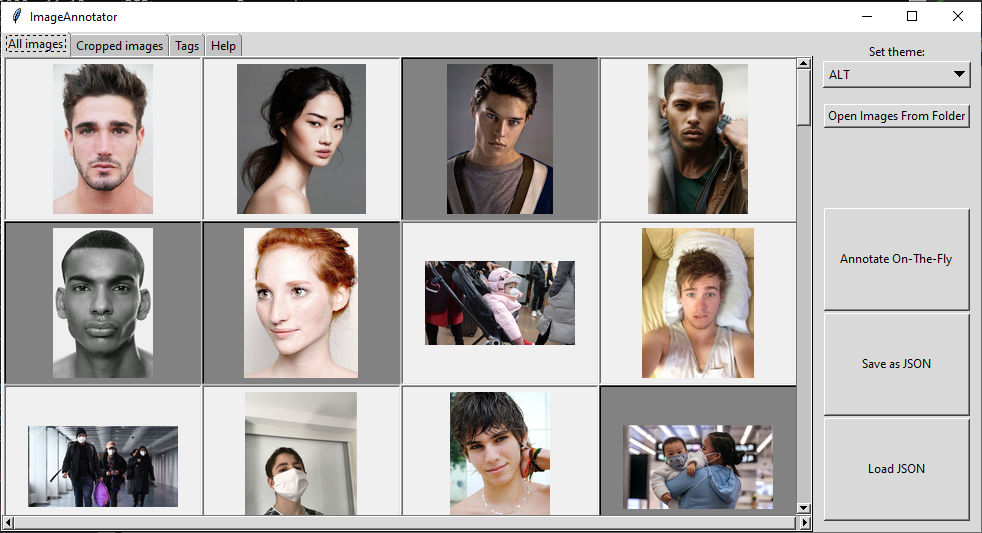
\includegraphics[width=1.0\textwidth]{images_latex/All_images.png}
    \caption{"All images" panel preview}
    \label{fig:all_img_panel}
\end{figure}

When we run the project, we can see the first panel shown is something similar to Figure \ref{fig:all_img_panel} where all images of the \textit{img} folder are displayed.
Here we can click on an image to open the \textit{annotator} panel.
\subsection{The annotator}
\begin{figure}
    \centering
    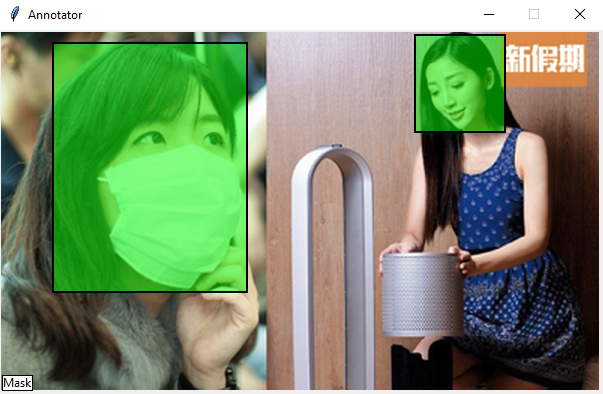
\includegraphics[width=1.0\textwidth]{images_latex/Annotator.png}
    \caption{Annotator preview}
    \label{fig:annotator_preview}
\end{figure}

From the annotator window, you can draw the rectangle representing a new annotation (in case of miss-click you can press the \textit{ESCAPE} button of the keyboard to undo the annotation drawing).

\begin{figure}%
    \centering
    \begin{subfigure}{4cm}
        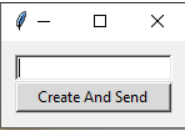
\includegraphics[width=\linewidth]{images_latex/Empty_tag.png}
        \caption{No existing tags}
        \label{fig:no_tag}
    \end{subfigure}
    \qquad
    \begin{subfigure}{4cm}
        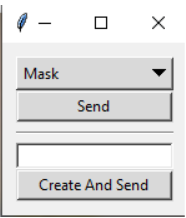
\includegraphics[width=\linewidth]{images_latex/Tag_choice.png}
        \caption{Scroll menu with tag}
        \label{fig:scrol_tag}
    \end{subfigure}
    \caption{Tag attribution}%
    \label{fig:tag_attrib}%
\end{figure}

Once the annotation drawn, you will see either the Figure \ref{fig:no_tag} when you still have not entered a tag or Figure \ref{fig:scrol_tag} offering you the possibility to choose an existing tag.

You are also able to rename or delete an existing annotation with the right key of the mouse. 
This will perform a simple rename of the tag for the current image and not a whole rename of a tag \textit{T1} in tag \textit{T2} (this task can be accomplished in the Tag Panel).

To know the name of an annotation you can move the mouse on it and a little tool-tip will display in the bottom-left corner of the annotator window.

Finally, if you create a box that does not respect the parameter imposed (area size, sides length or covering constraints of Listing \ref{listing:ann_constraints}) an error message will be prompt to warn you about the impossibility of performing this task.

\subsection{The cropped images panel}

\begin{figure}
    \centering
    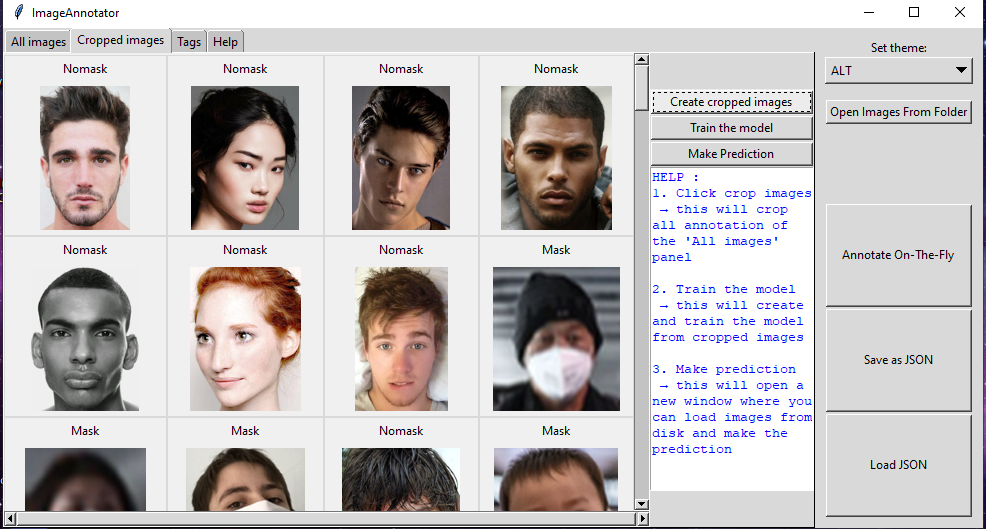
\includegraphics[width=1.0\textwidth]{Cropped_images.png}
    \caption{Cropped image panel}
    \label{fig:cropped_img_panel}
\end{figure}

The cropped panel (see \ref{fig:cropped_img_panel}) is the panel which aims to create the model of neural network by which you will make you prediction.

In this panel, after having annotate the images you want, you click on \textit{Create cropped images} button to crop and resize all annotations. In this panel you will see a miniature of all annotations associated with the name of the tag you gave.

Then you can \textit{Train the model}. This is the core earth of our project, we will explain more about our model decisions in Section \ref{sec:model}.

\begin{figure}
    \centering
    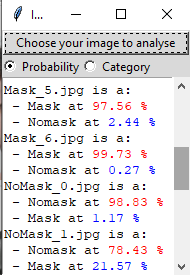
\includegraphics[width=4cm]{images_latex/Prediction.png}
    \caption{Predictor preview}
    \label{fig:pred}
\end{figure}

Once the model created, you can click \textit{Make prediction} button and in the new opened window (see \ref{fig:pred}) you can choose the images on which you want to make a prediction (you can choose multiple files in a folder).

\subsection{The tag panel}

This panel is composed of a grid of existing tags and the \textit{Add tag} button.

You can add a tag via the corresponding button and rename or delete an existing one by right-clicking on it (in this case the rename will impact every image's annotation).

\subsection{The help panel}

The help panel contains a brief description on how our interface works and it is composed of four clickable buttons, each of them showing its related text. 

\subsection{The right panel}

\begin{wrapfigure}{r}{5.5cm}
    \centering
    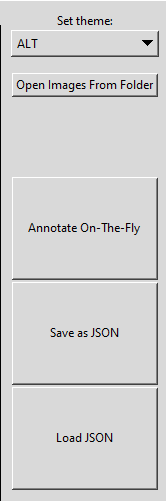
\includegraphics[width=3cm]{Right_panel.png}
    \caption{Right panel preview}
    \label{fig:rgt_panel}
\end{wrapfigure}

The right panel of our interface contains some buttons performing different tasks.

You can modify the theme of the window via the \textit{OptionMenu} under the \textit{"Set theme"} label.

The other buttons:
\begin{itemize}
    \item Open images From Folder: allows you to load the images from a chosen folder.
    \item Annotate On-The-Fly: allows you to load a single image and make annotations on it. You can then save these annotations in the folder you want thanks to the button \textit{Save}.
  \item Load JSON (resp. Save as JSON): allows you to load (resp. save) a JSON file with the annotations of current (resp. previous) session.
\end{itemize}

\section{Models}
\label{sec:model}

Training a neural network revolves around three main objects:

\begin{itemize}
    \item \textit{Layers}
    \item \textit{Loss function}
    \item \textit{Optimizer}
\end{itemize}

\subsection{Layers}

The core building block of neural networks is the layer, which is a \textit{"data-processing module that you can think of as a filter for data"}\supercite{nnlbook}.

The function of a layer is to extract the representation of the data which are fed into them. 
Most of deep learning are characterized by a chain of simple layers.

\begin{lstlisting}[
    caption={Layer code example},
    label={listing:lay_code_ex},
    mathescape=true, 
    frame=lines,
     breaklines=true,
    backgroundcolor=\color{yellow!25},
]
model  = keras.models.Sequential([
    data_augmentation,
    layers.Rescaling(1./255),
    layers.Conv2D(16, 3, padding='same', activation='relu'),
    layers.MaxPooling2D(),
    layers.Dropout(0.2),
    layers.Flatten(),
    layers.Dense()
])
\end{lstlisting}

Now let's see the different layers taken in account in our models :
\begin{itemize}
    \item\textit{Rescaling}: it rescale the pixels value (between 0 and 255) to the [0,1] interval. 
    \item\textit{Conv2D}: is the layer to convolve the image into multiple images. It takes as input tensors of shape and is defined by two key parameters: the \textit{depth of the output feature map} and the \textit{size of the patches extracted from the inputs}. 
    \item\textit{MaxPooling}: is used to extracting window from the input feature maps and outputting the max value of each channel.
    \item\textit{Dropout}: it set to 0 (= \textit{dropping out}) a number of output features of the layer during training. It is usually used to avoid overfitting. It is usually set between 0.2 and 0.5.
    \item\textit{Flatten}: is used to flatten the dimension of the image obtained after convolving it.
    \item\textit{Dense}: it is the hidden layer in which there are the hidden units of the layer.
\end{itemize}

\subsection{Loss function and optimizer}

The \textit{loss function} defines the feedback signal used for learning, it is necessary to measure the performance on the training data and it is part of the compilation step of the model.

The \textit{optimizer}, which is also located in the compilation step, is a mechanism through which the network will update itself based on the loss function.

\section{Overfitting and underfitting}
A model is underfit when, at the beginning of training, optimization and generalization are correlated. In this case, the network hasn't yet modeled all relevant patterns. 

A model starts to overfit when a certain number of iterations are made, generalization stop improving and validation metrics stall and then begin to degrade. 

To prevent the overfitting in neural networks usually the following methods are used: 

\begin{itemize}
    \item get more training data
    \item reduce the capacity of the network
    \item add weight regularization
    \item add dropout.
\end{itemize}

\section{Our models}
In this section we are going to observe and compare the models we have analyzed to create our neuronal network system (each model has been tested for 3 times). 

\subsection{How to read the following charts}
We represent some model result by a bar chart where green bars represent a correct result and red bars a false result to see how a model works.

Every model is then associated with another graph containing an average of the found results. We have information about True Positive (the \textit{Mask} case), False positive, True negative (the \textit{NoMask} case) and False negative. The percentage represent the mean of the statistics that we could deduce from multiple iterations on the same model, a good model is the one where the sum of values of the True column (the green zone) is as big as possible.

\newpage
\subsection{Model 1}
\begin{lstlisting}[
    caption={Model 1},
    label={listing:mod_1},
    mathescape=true, 
    frame=lines,
     breaklines=true,
    backgroundcolor=\color{yellow!25},
]
 model = keras.models.Sequential([
    data_augmentation,
    layers.Rescaling(1./255), 
    layers.Conv2D(16, 3, padding='same', activation='relu'),
    layers.MaxPooling2D(2),
    layers.Conv2D(32, 3, padding='same', activation='relu'),
    layers.MaxPooling2D(),
    layers.Conv2D(64, 3, padding='same', activation='relu'),
    layers.MaxPooling2D(),
    layers.Dropout(0.2),
    layers.BatchNormalization(), 
    layers.Flatten(),
    layers.Dense(num_classes)
])
\end{lstlisting}
   
\textbf{Model 1 results}

\begin{figure}%
    \centering
    \begin{subfigure}{6cm}
        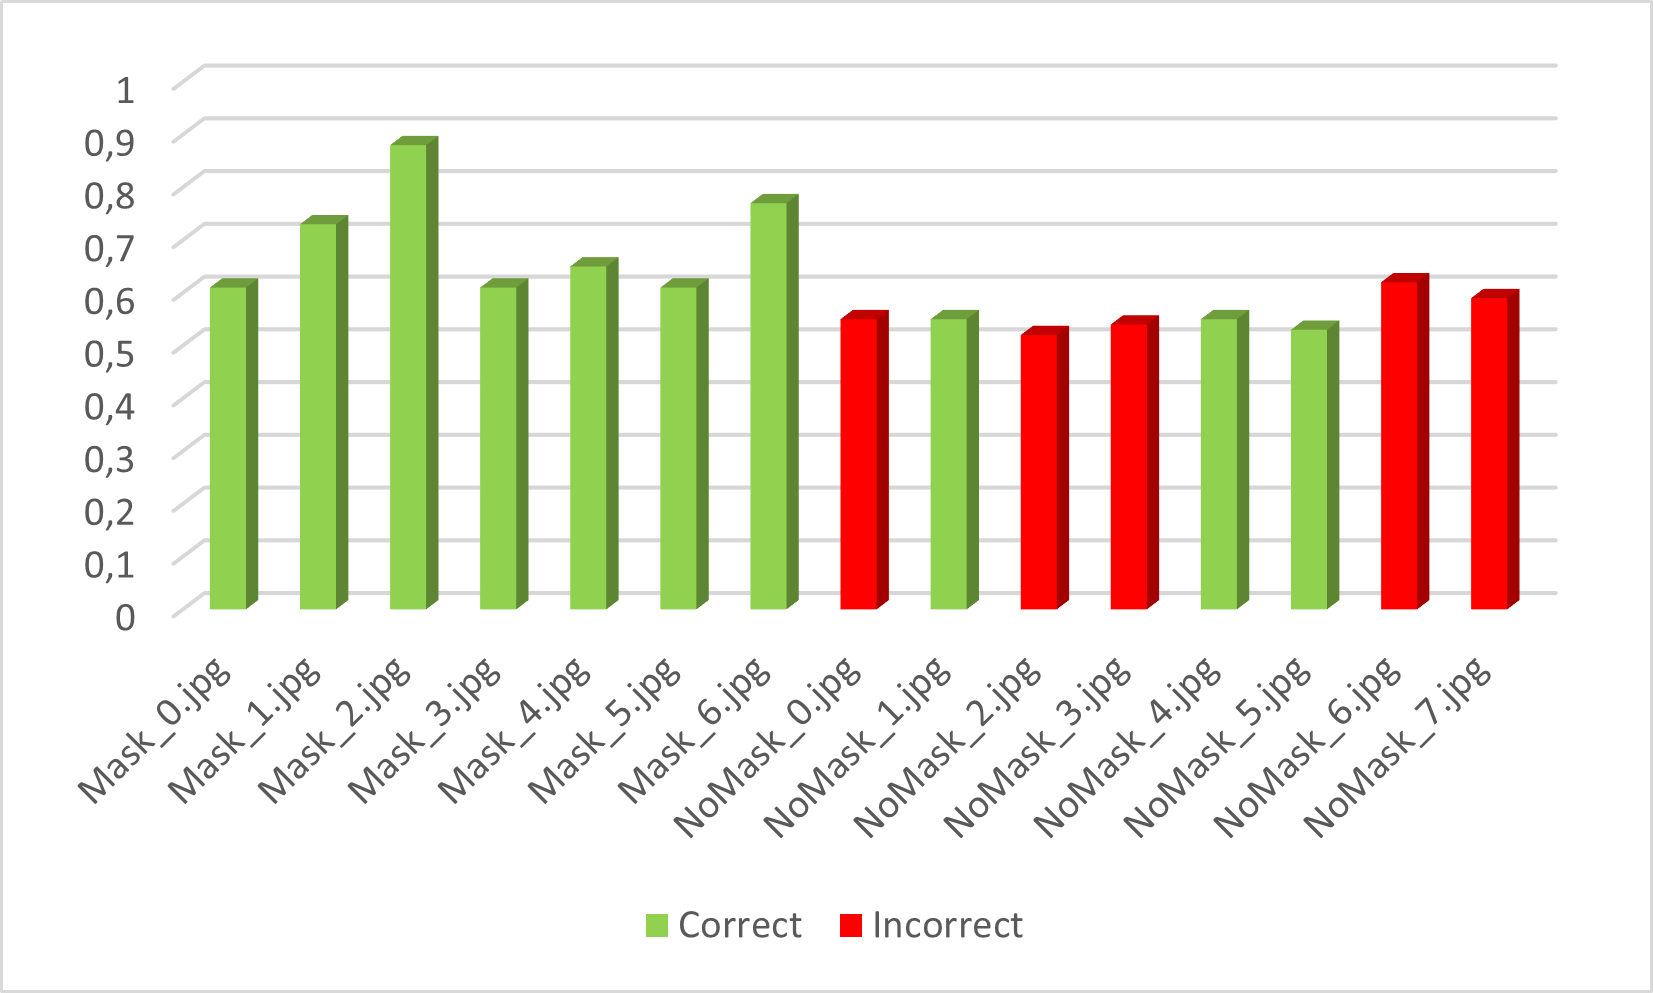
\includegraphics[width=\linewidth]{images_latex/test1_1.png}
        \caption{Model 1 - Test 1}
    \end{subfigure}
    \qquad
    \begin{subfigure}{6cm}
        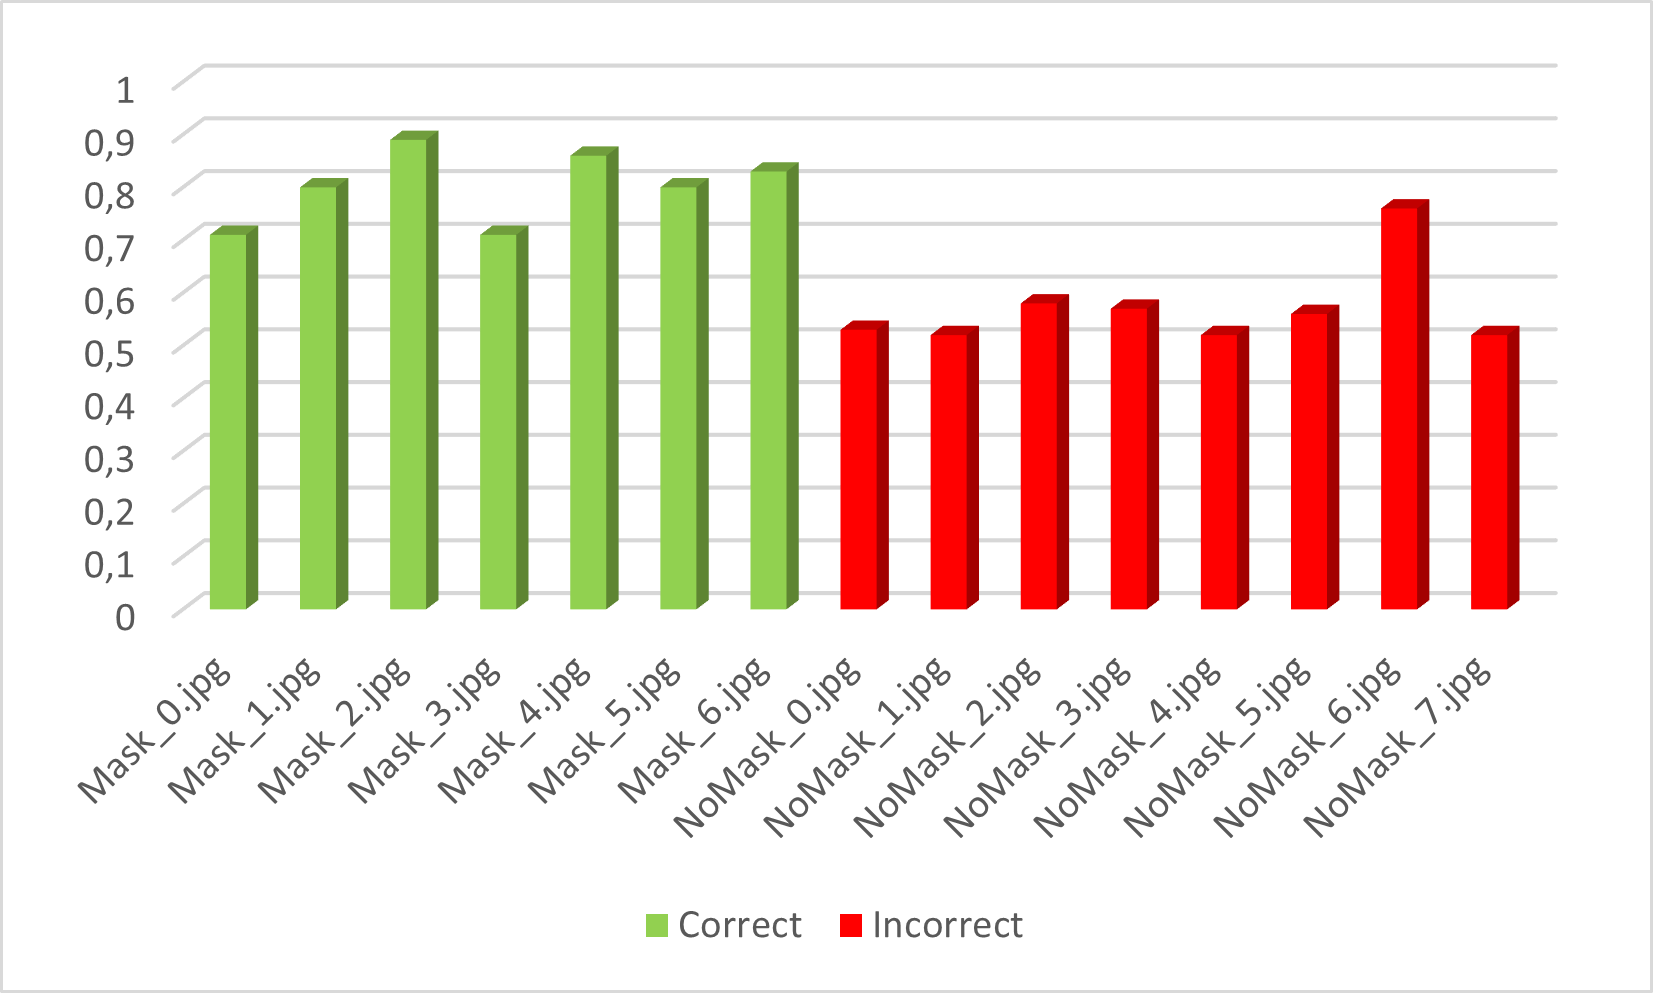
\includegraphics[width=\linewidth]{images_latex/test1_2.png}
        \caption{ Model 1 - Test 2}
    \end{subfigure}
    \qquad
    \begin{subfigure}{6cm}
        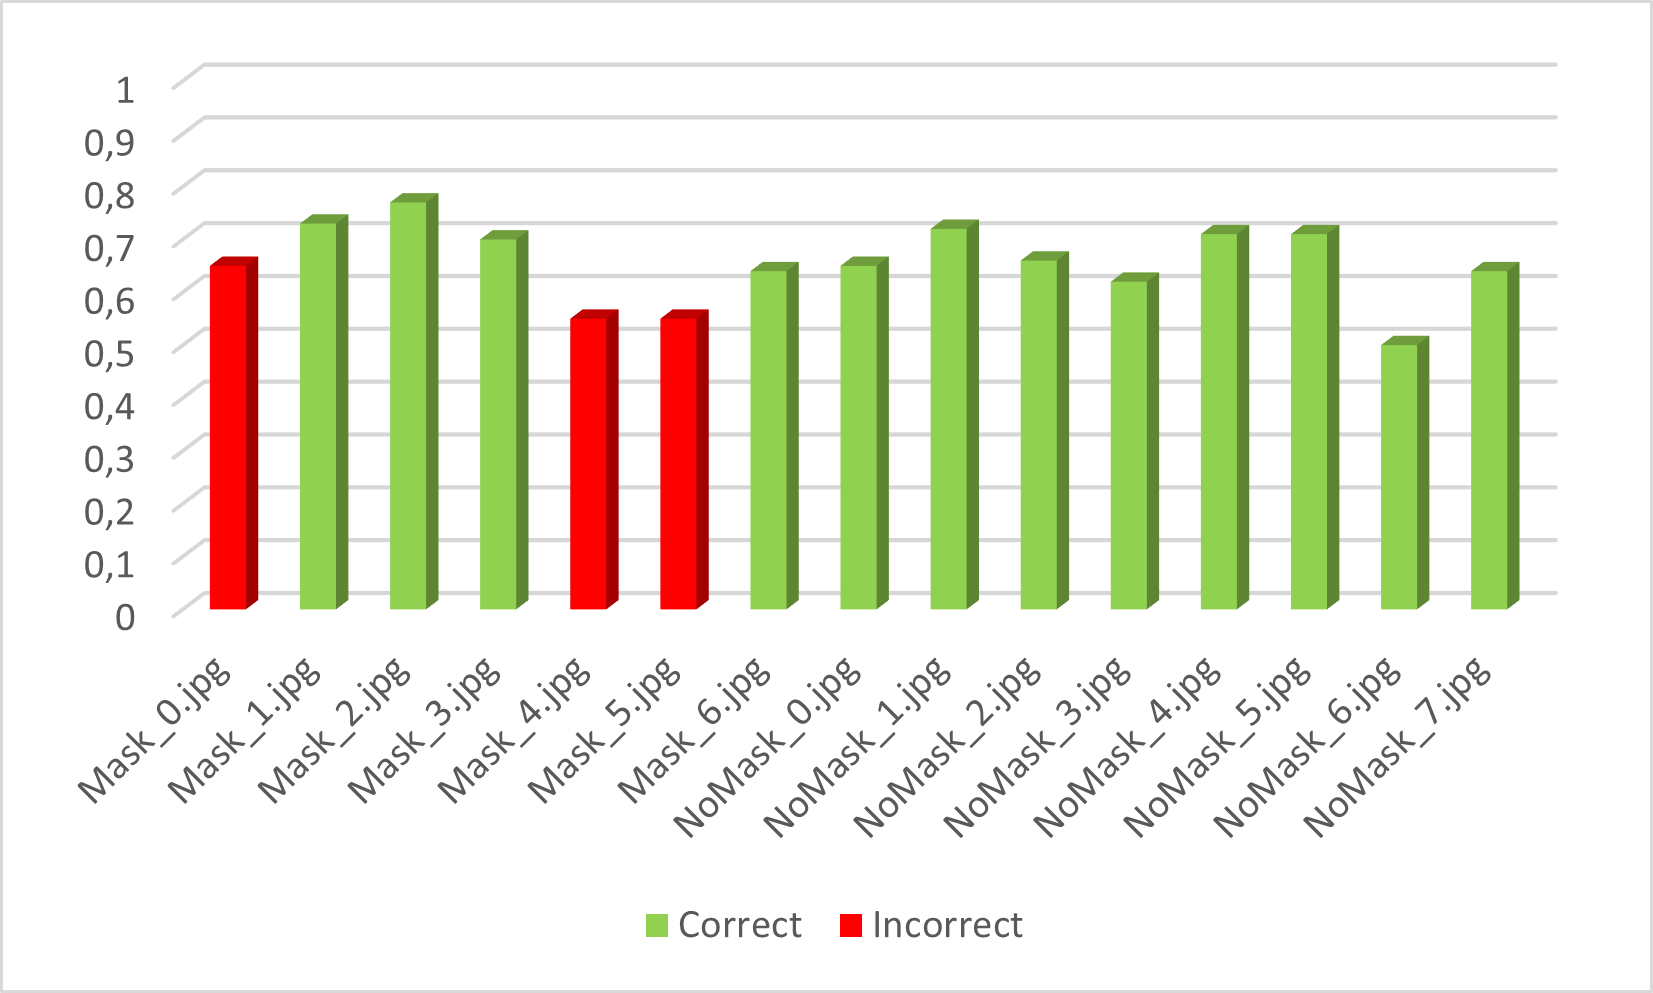
\includegraphics[width=\linewidth]{images_latex/test1_3.png}
        \caption{ Model 1 - Test 3}
    \end{subfigure}
     \begin{subfigure}{6cm}
        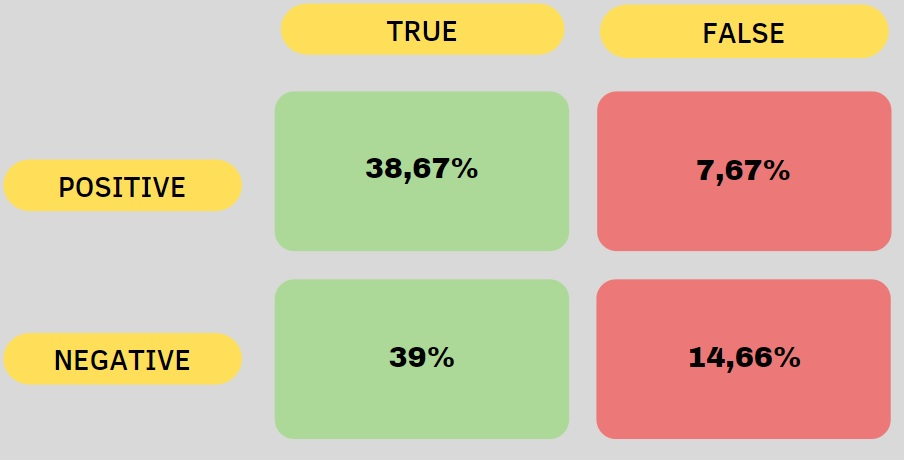
\includegraphics[width=\linewidth]{images_latex/model1.jpg}
        \caption{ Model 1 - Prediction}
    \end{subfigure}
    \caption{Scenario 1}%
    \label{fig:mod_1_tests}
\end{figure}

We started setting up three Conv2D layers with three different number of channels and one of the MaxPooling to 2.
As we can deduce from three images \ref{fig:mod_1_tests}, this model isn't a good model. 
It can't recognise very well in which image there is a mask and the probability percentage is low. 
\newpage
\subsection{Model 2}
\begin{lstlisting}[
    caption={Model 2},
    label={listing:mod_2},
    mathescape=true, 
    frame=lines,
     breaklines=true,
    backgroundcolor=\color{yellow!25},
]
model = keras.models.Sequential([
   data_augmentation,
   layers.Rescaling(1./255), 
   layers.Conv2D(128, 3, padding='same',activation='relu'),
   layers.MaxPooling2D(2),
   layers.Conv2D(32, 3, padding='same', activation='relu'),
   layers.MaxPooling2D(),
   layers.Dropout(0.2),
   layers.BatchNormalization(), 
   layers.Flatten(),
   layers.Dense(num_classes)
])
\end{lstlisting}
    
\textbf{Model 2 results}

\begin{figure}%
    \centering
    \begin{subfigure}{6cm}
        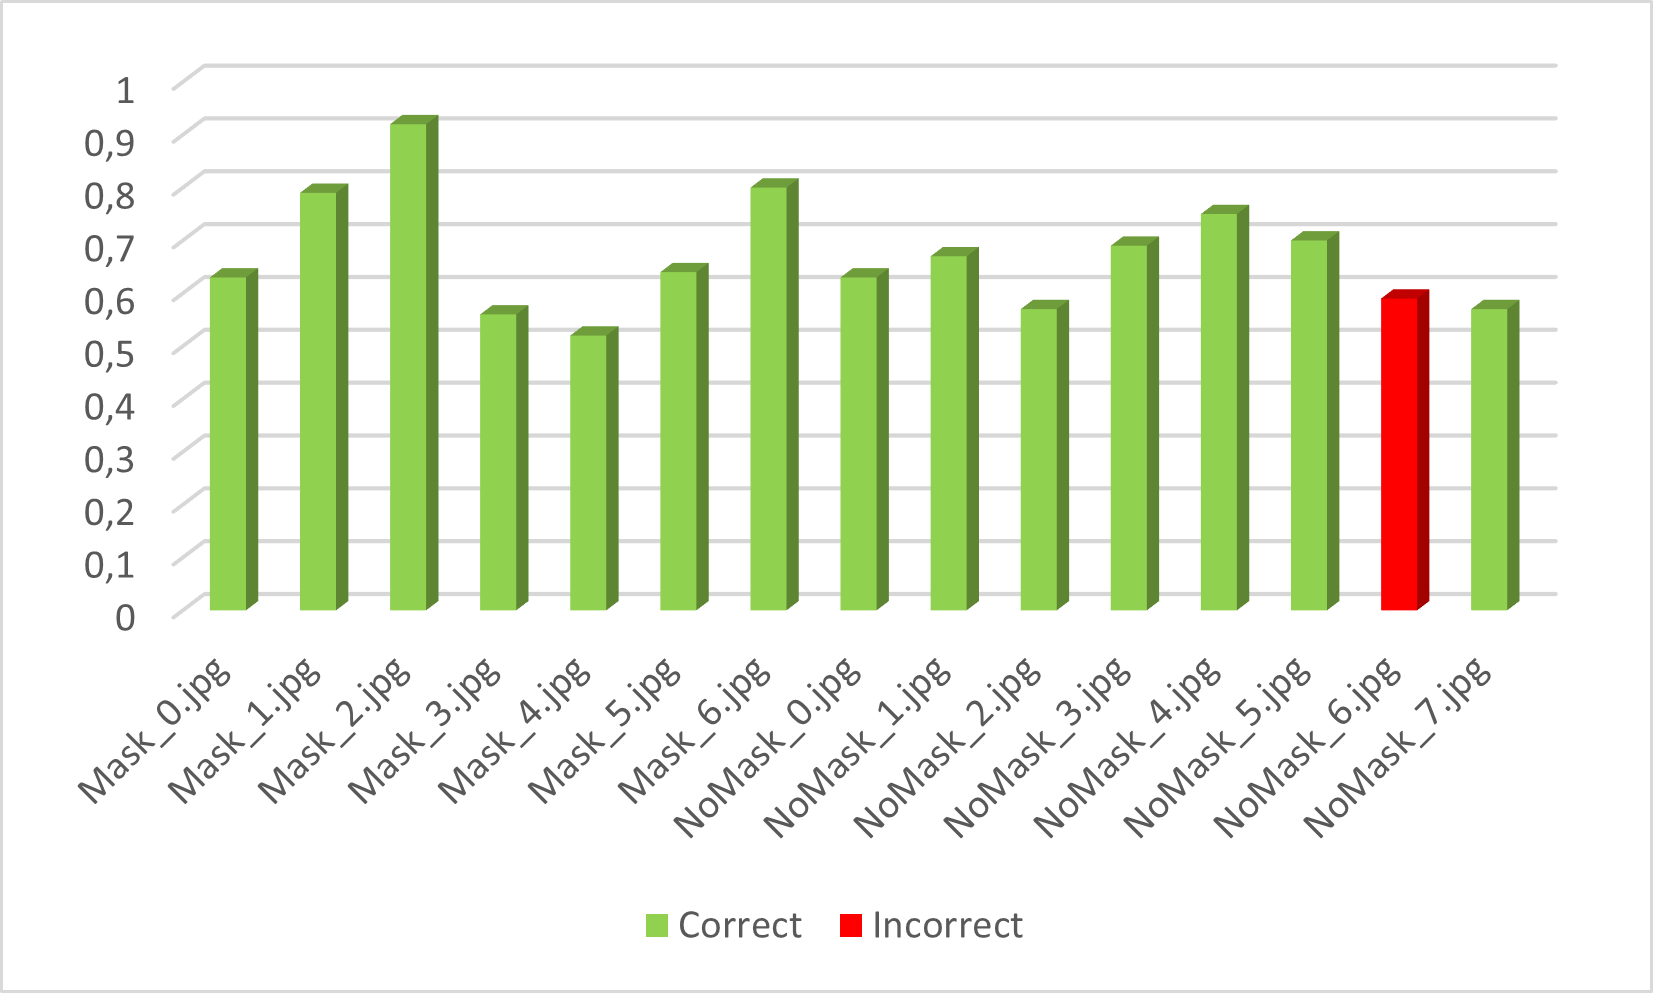
\includegraphics[width=\linewidth]{images_latex/test2_1.png}
        \caption{Model 2 - Test 1}
        \label{fig:t2_1}
    \end{subfigure}
    \qquad
    \begin{subfigure}{6cm}
        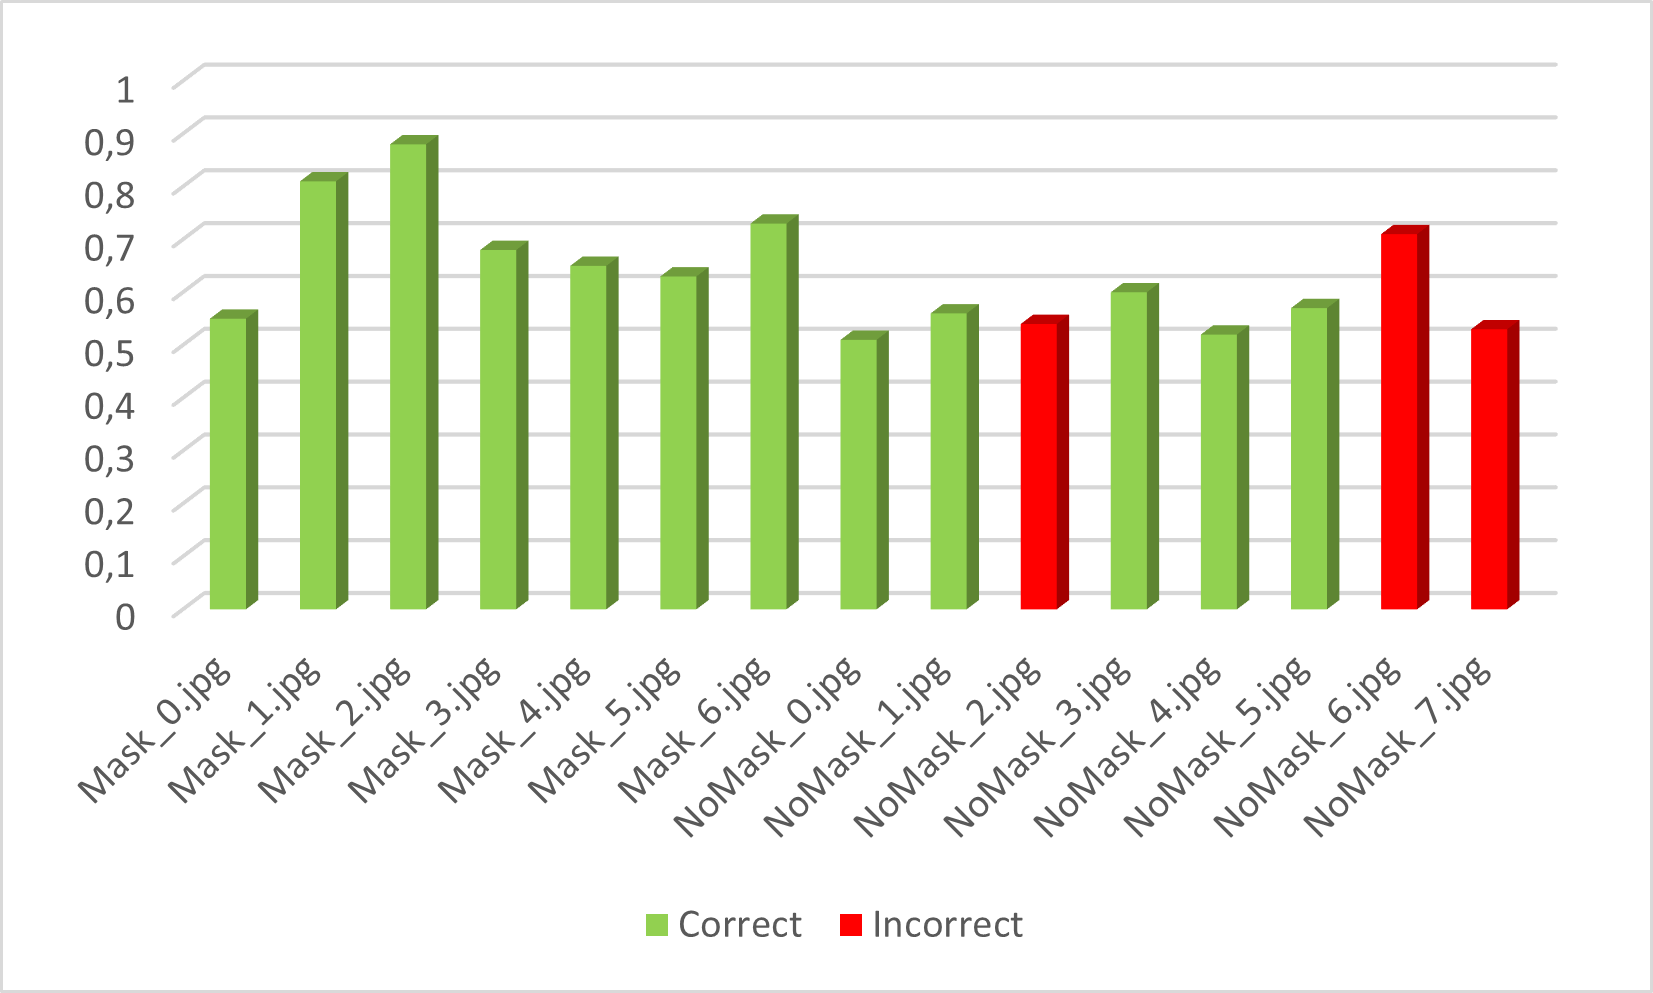
\includegraphics[width=\linewidth]{images_latex/test2_2.png}
        \caption{ Model 2 - Test 2}
    \end{subfigure}
    \qquad
    \begin{subfigure}{6cm}
        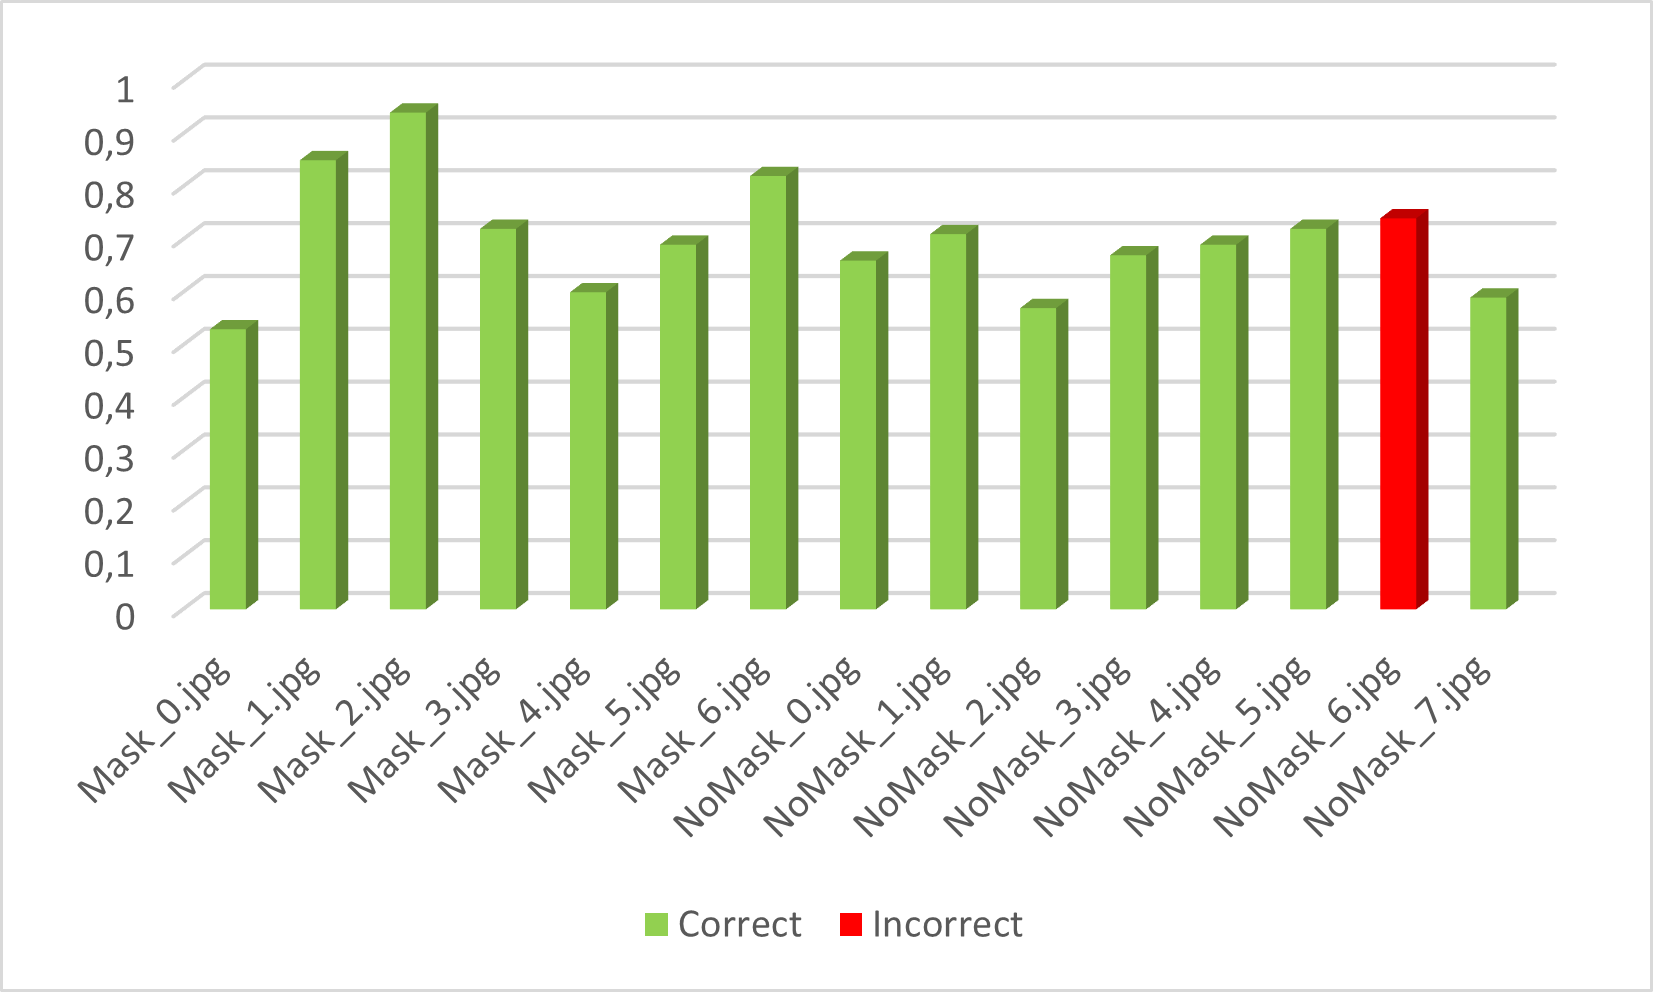
\includegraphics[width=\linewidth]{images_latex/test2_3.png}
        \caption{ Model 2 - Test 3}
    \end{subfigure}
    \begin{subfigure}{6cm}
        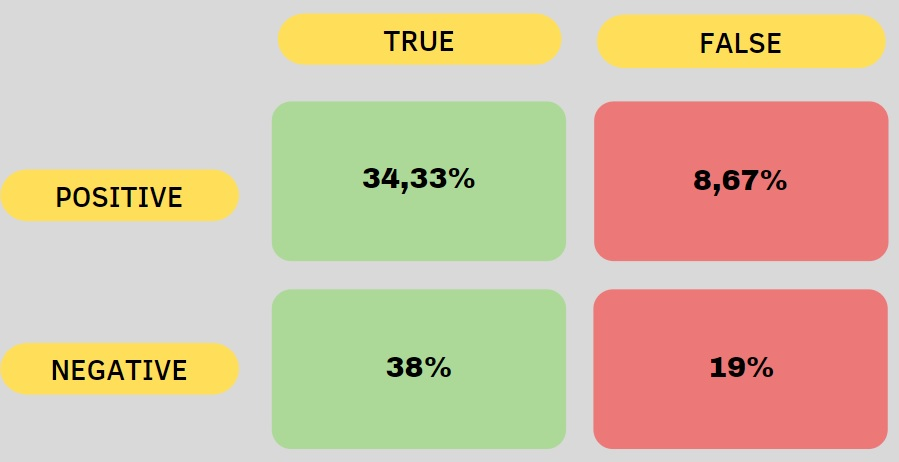
\includegraphics[width=\linewidth]{images_latex/model2.jpg}
        \caption{ Model 2 - Prediction}
    \end{subfigure}
    \caption{Scenario 2}
\end{figure}

For this model we chose to set up two Conv2D layers (one of them with an higher number of channels) leaving unchanged the other layers. 

The result is a better model then the previous one; for example, in Figure \ref{fig:t2_1}, you can see that the recognition of the Mask/Nomask images is correct but the probability percentage is still low. 
\newpage
\subsection{Model 3}
\begin{lstlisting}[
    caption={Model 3},
    label={listing:mod_3},
    mathescape=true, 
    frame=lines,
     breaklines=true,
    backgroundcolor=\color{yellow!25},
]
model = keras.models.Sequential([
    data_augmentation,
    layers.Rescaling(1./255), 
    layers.Conv2D(128, 3, padding='same', activation='relu'),
    layers.MaxPooling2D(4),
    layers.Conv2D(64, 3, padding='same', activation='relu'),
    layers.MaxPooling2D(),
    layers.Dropout(0.4),
    layers.BatchNormalization(), 
    layers.Flatten(),
    layers.Dense(num_classes)
])
\end{lstlisting}

\textbf{Results}

\begin{figure}%
    \centering
    \begin{subfigure}{6cm}
        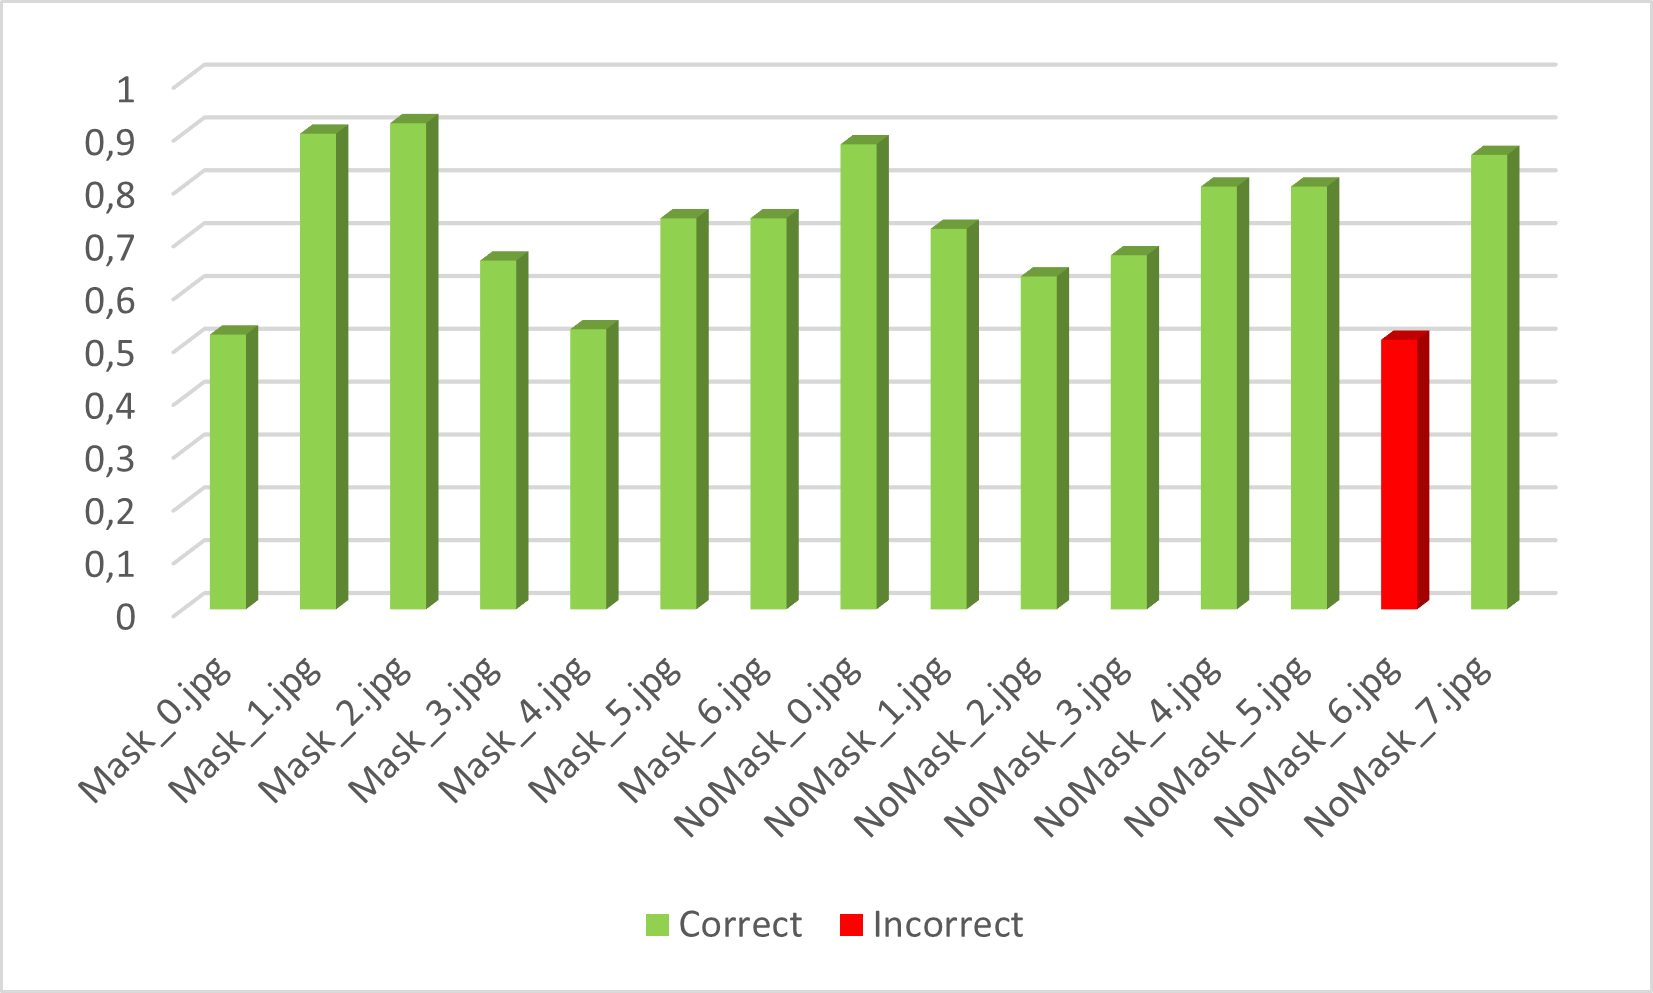
\includegraphics[width=\linewidth]{images_latex/test3_1.png}
        \caption{Model 3 - Test 1}
        \label{fig:t3_1}
    \end{subfigure}
    \qquad
    \begin{subfigure}{6cm}
        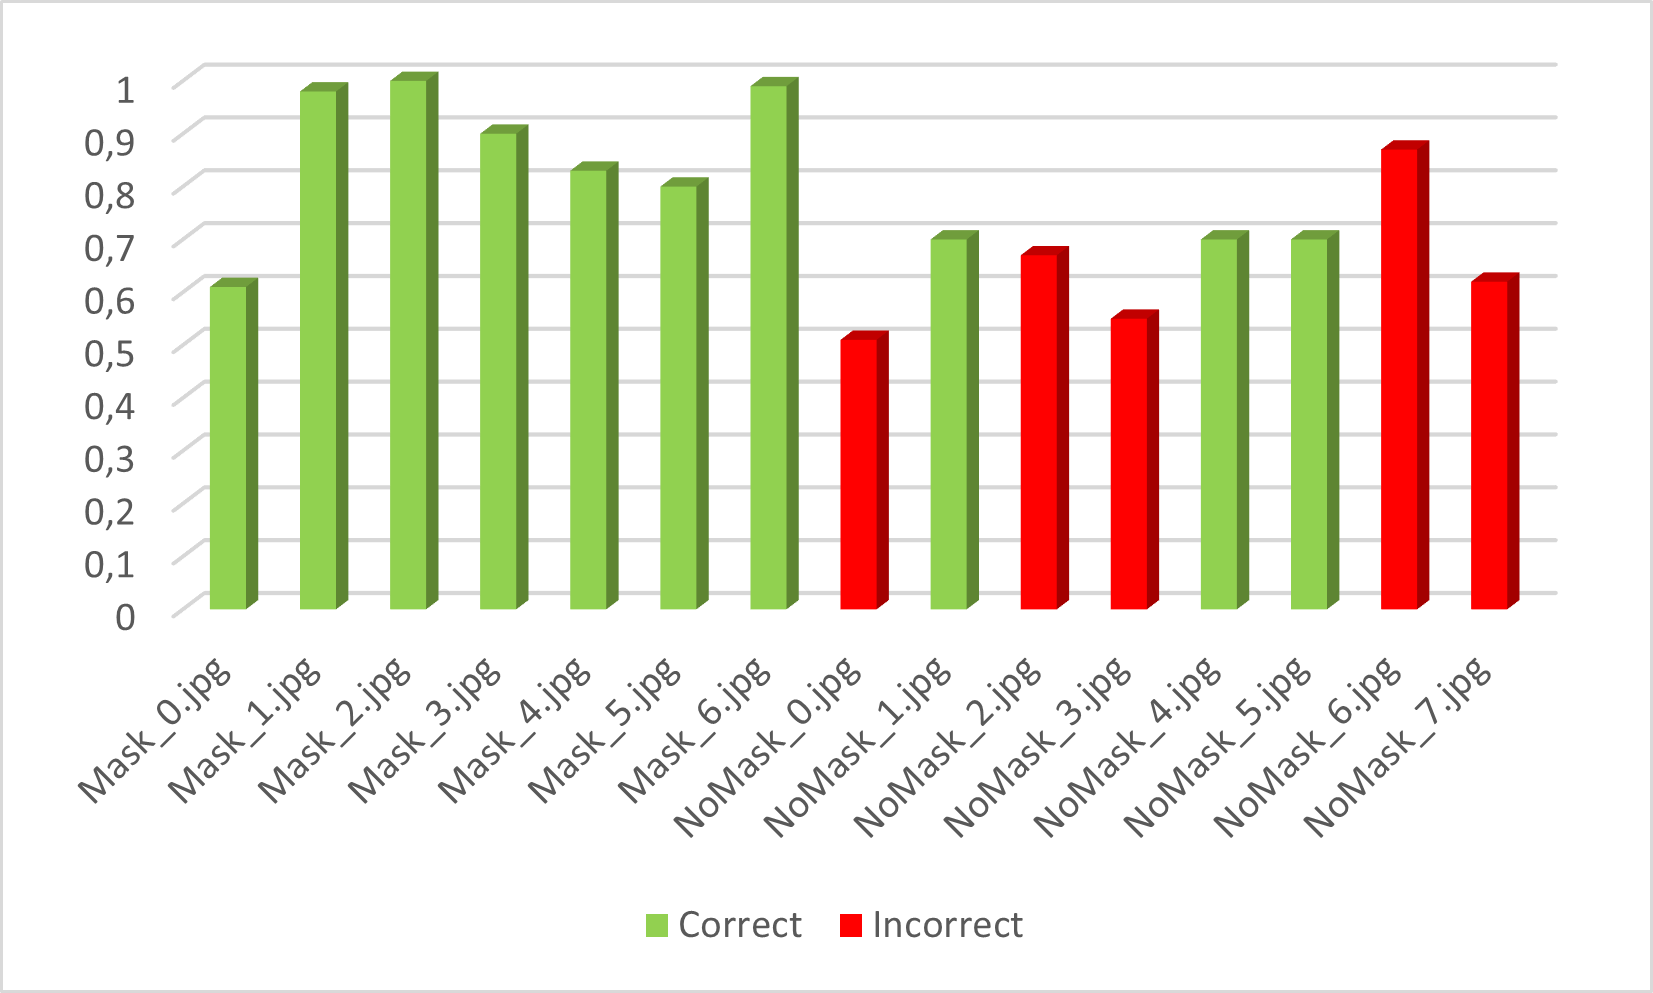
\includegraphics[width=\linewidth]{images_latex/test3_2.png}
        \caption{ Model 3 - Test 2}
    \end{subfigure}
    \qquad
    \begin{subfigure}{6cm}
        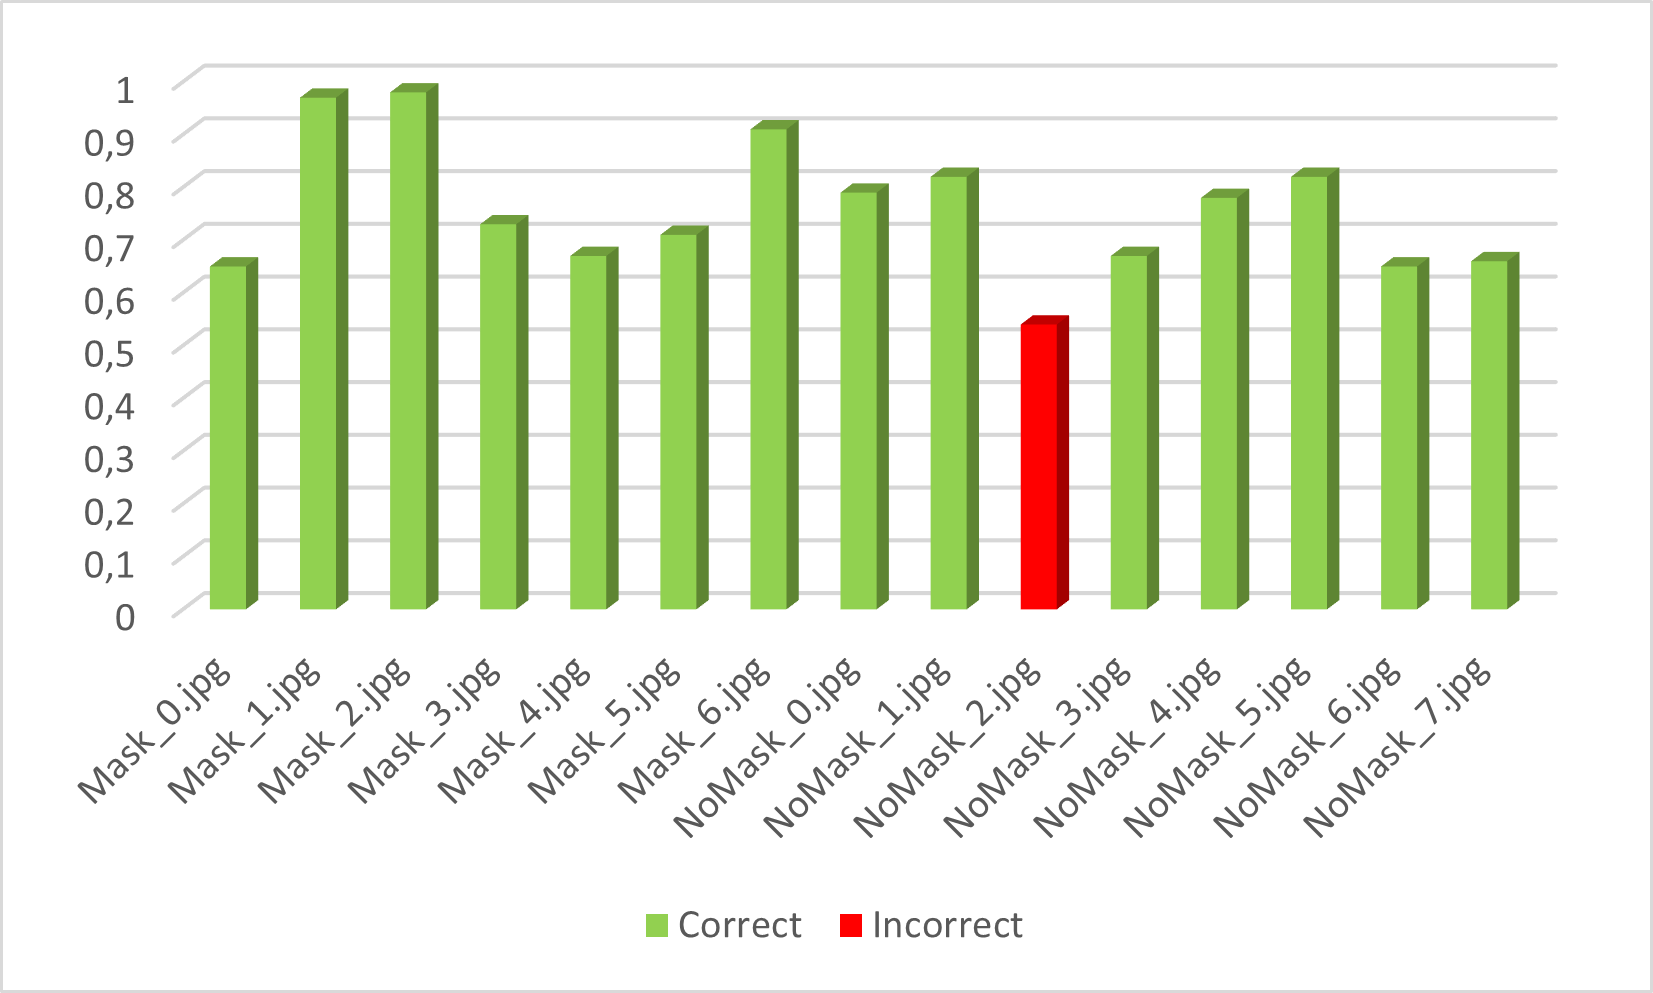
\includegraphics[width=\linewidth]{images_latex/test3_3.png}
        \caption{ Model 3 - Test 3}
    \end{subfigure}
     \begin{subfigure}{6cm}
        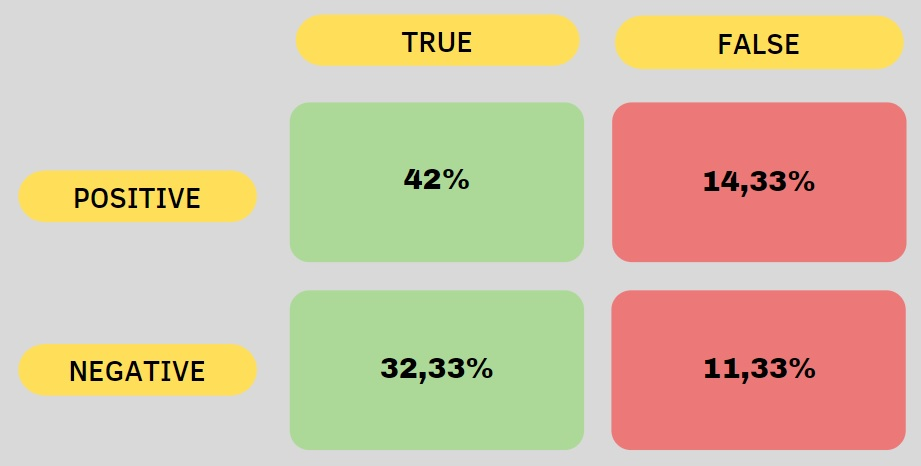
\includegraphics[width=\linewidth]{images_latex/model3.jpg}
        \caption{ Model 3 - Prediction}
    \end{subfigure}
    \caption{Scenario 3}%
\end{figure}

With this model we decided to keep the same number of layers, changing some of their parameters, such as the number of channels of Conv2D layers and the parameters of the first MaxPooling and the Dropout. 
In this case it seems to be better then the second as regards the percentages, but it still remains a model that can be excluded. 

\newpage
\subsection{Model 4}
\begin{lstlisting}[
    caption={Model 4},
    label={listing:mod_4},
    mathescape=true, 
    frame=lines,
     breaklines=true,
    backgroundcolor=\color{yellow!25},
]
model = keras.models.Sequential([
    data_augmentation,
    layers.Rescaling(1./255), 
    layers.Conv2D(16, 3, padding='same', activation='relu'),
    layers.MaxPooling2D(2),
    layers.Conv2D(32, 3, padding='same', activation='relu'),
    layers.MaxPooling2D(2),
    layers.Conv2D(64, 3, padding='same', activation='relu'),
    layers.MaxPooling2D(),
    layers.Conv2D(128, 3, padding='same', activation='relu'),
    layers.MaxPooling2D(4),
    layers.Dropout(0.2),
    layers.BatchNormalization(), 
    layers.Flatten(),
    layers.Dense(num_classes)
])
\end{lstlisting}

\textbf{Results}

\begin{figure}%
    \centering
    \begin{subfigure}{6cm}
        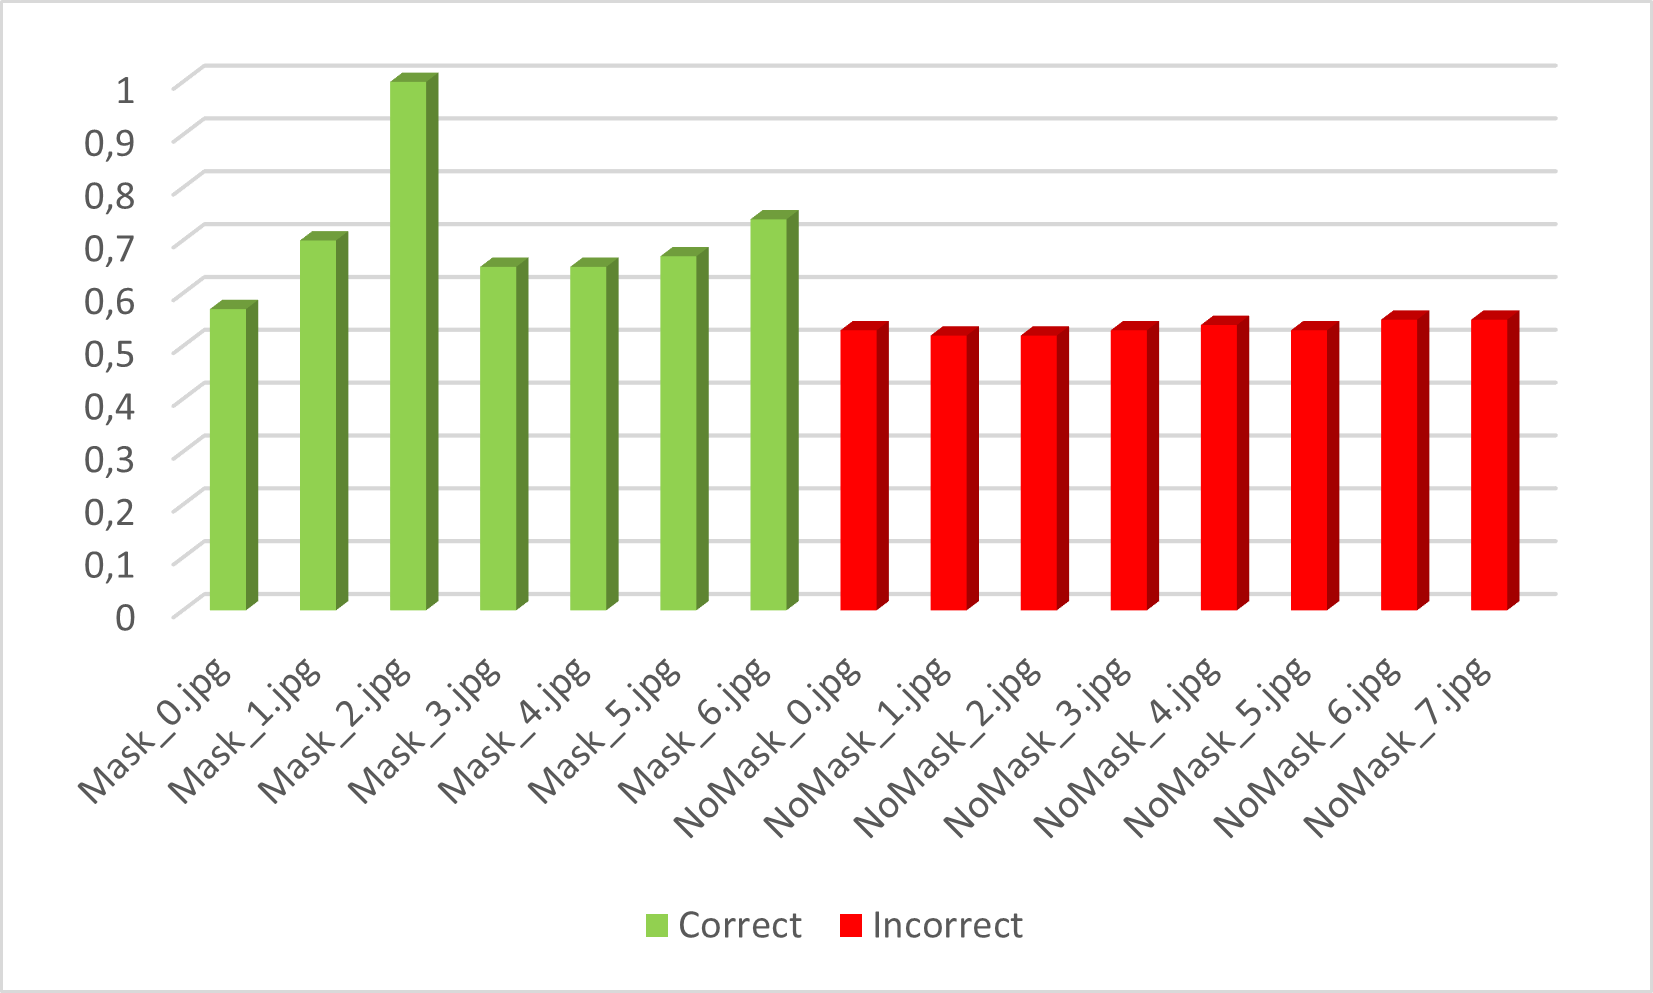
\includegraphics[width=\linewidth]{images_latex/test4_1.png}
        \caption{Model 4 - Test 1}
    \end{subfigure}
    \qquad
    \begin{subfigure}{6cm}
        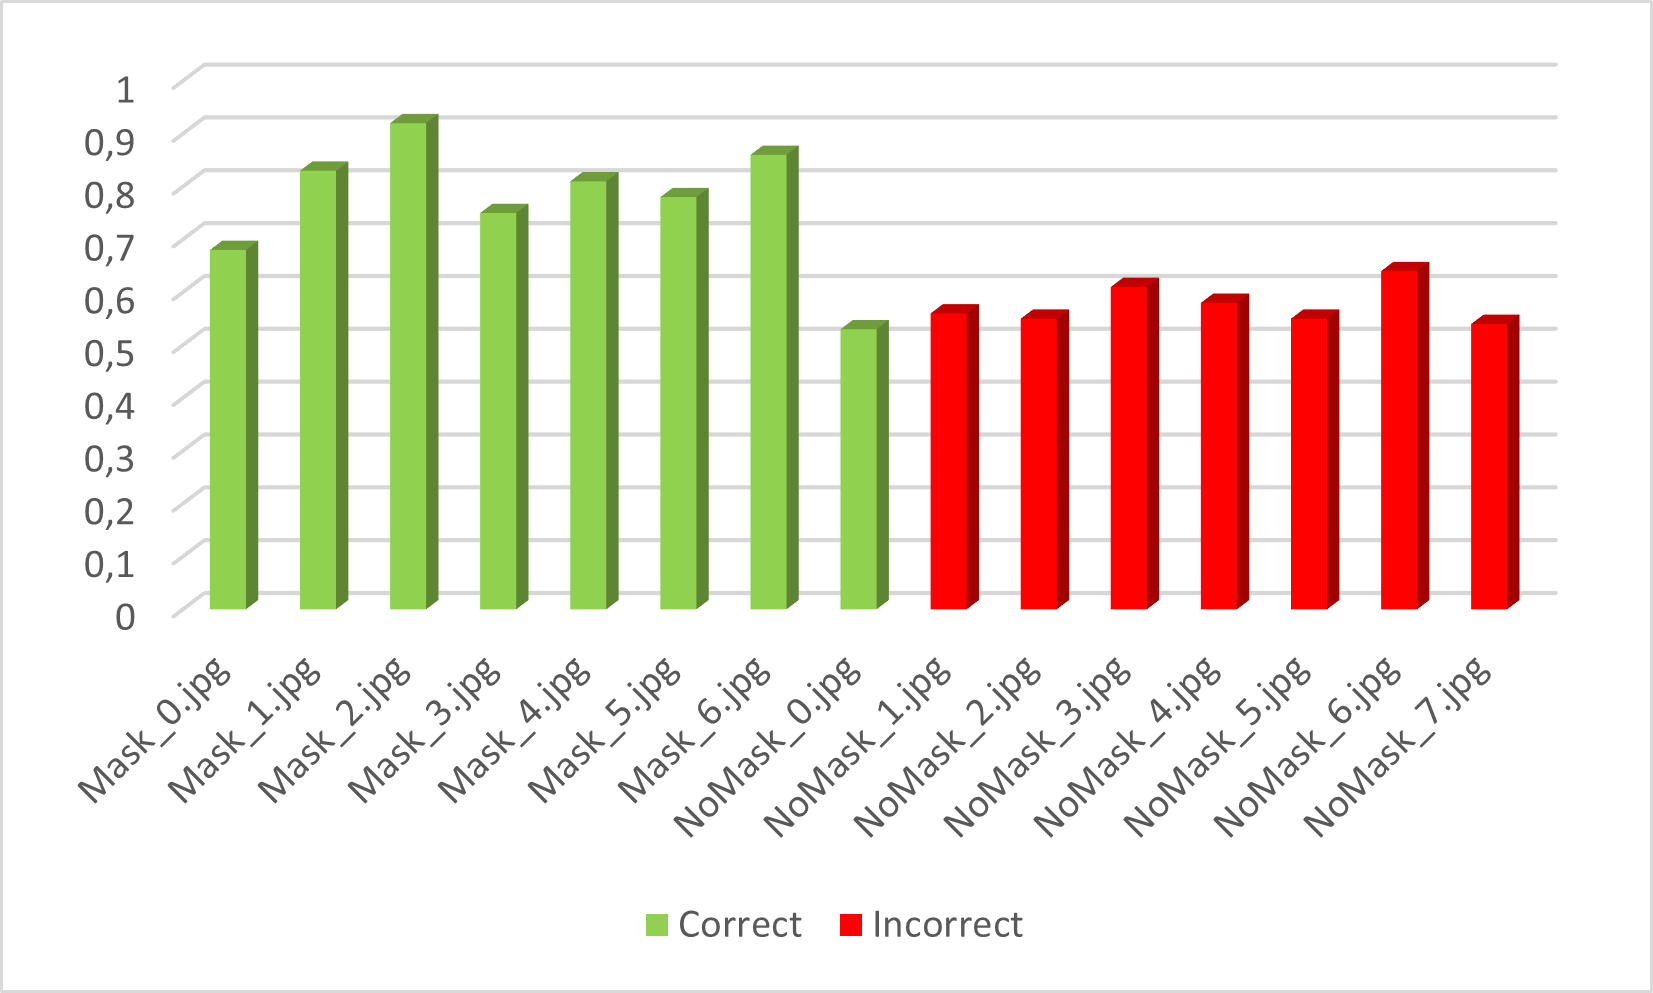
\includegraphics[width=\linewidth]{images_latex/test4_2.png}
        \caption{ Model 4 - Test 2}
    \end{subfigure}
    \qquad
    \begin{subfigure}{6cm}
        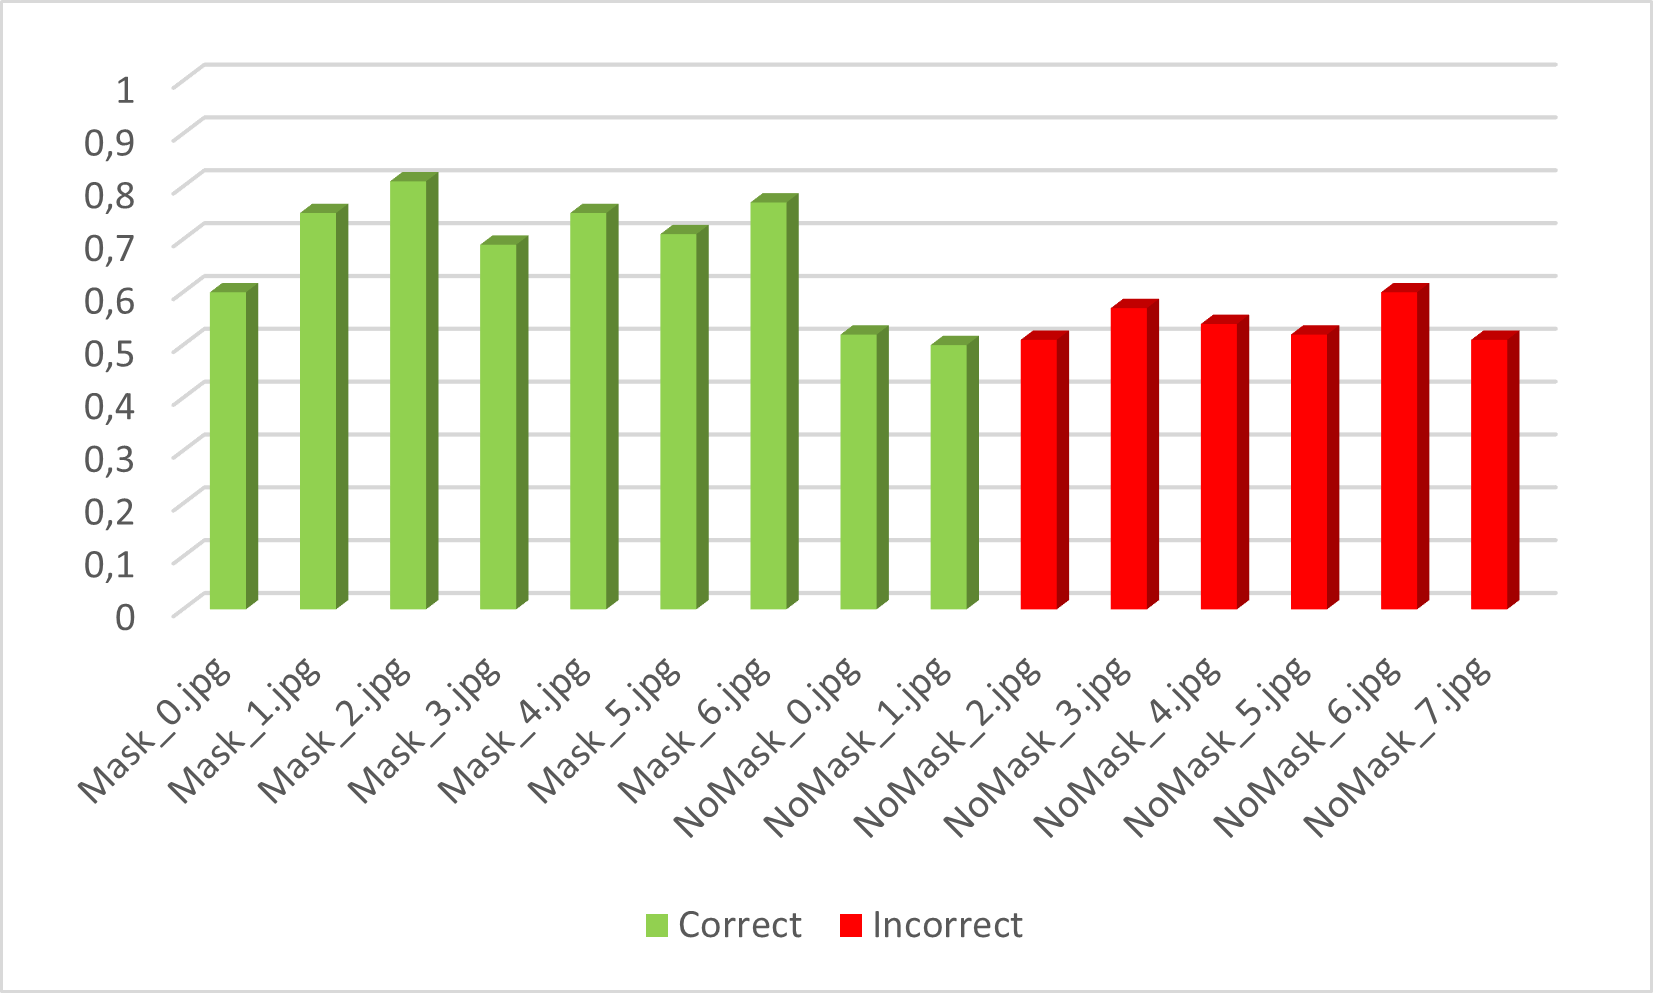
\includegraphics[width=\linewidth]{images_latex/test4_3.png}
        \caption{ Model 4 - Test 3}
    \end{subfigure}
     \begin{subfigure}{6cm}
        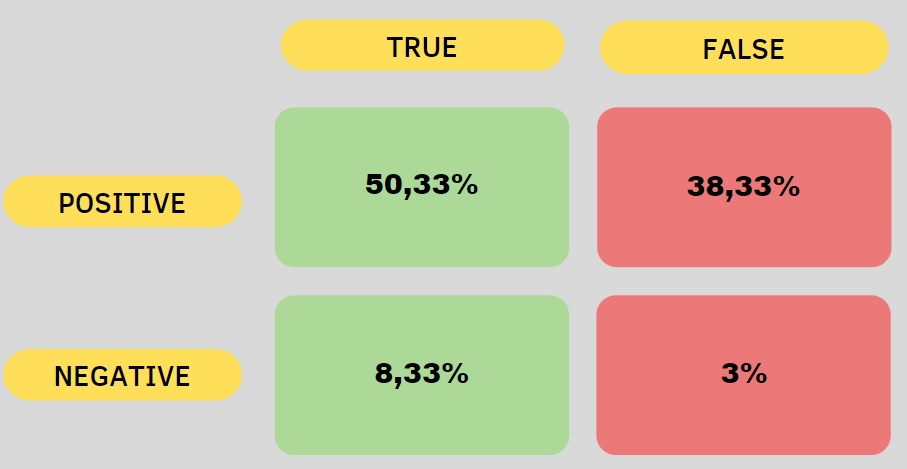
\includegraphics[width=\linewidth]{images_latex/model4.jpg}
        \caption{ Model 4 - Prediction}
    \end{subfigure}
    \caption{Scenario 4}%
\end{figure}

The fourth model involves new layers, in particular three Convs2d layers each with different values, ranging to the lowest to the highest. 
The result is the worst model, it gathers the mask category to almost all images.
\subsection{Model 5}
\begin{lstlisting}[
    caption={Model 5},
    label={listing:mod_5},
    mathescape=true, 
    frame=lines,
     breaklines=true,
    backgroundcolor=\color{yellow!25},
]
model  = keras.models.Sequential([
    data_augmentation,
    layers.Rescaling(1./255),
    layers.Conv2D(16, 3, padding='same', activation='relu'),
    layers.MaxPooling2D(),
    layers.Conv2D(16, 3, padding='same', activation='relu'),
    layers.MaxPooling2D(),
    layers.Dropout(0.2),
    layers.Flatten(),
    layers.Dense(num_classes)
])
\end{lstlisting}

\textbf{Results}

\begin{figure}%
    \centering
    \begin{subfigure}{6cm}
        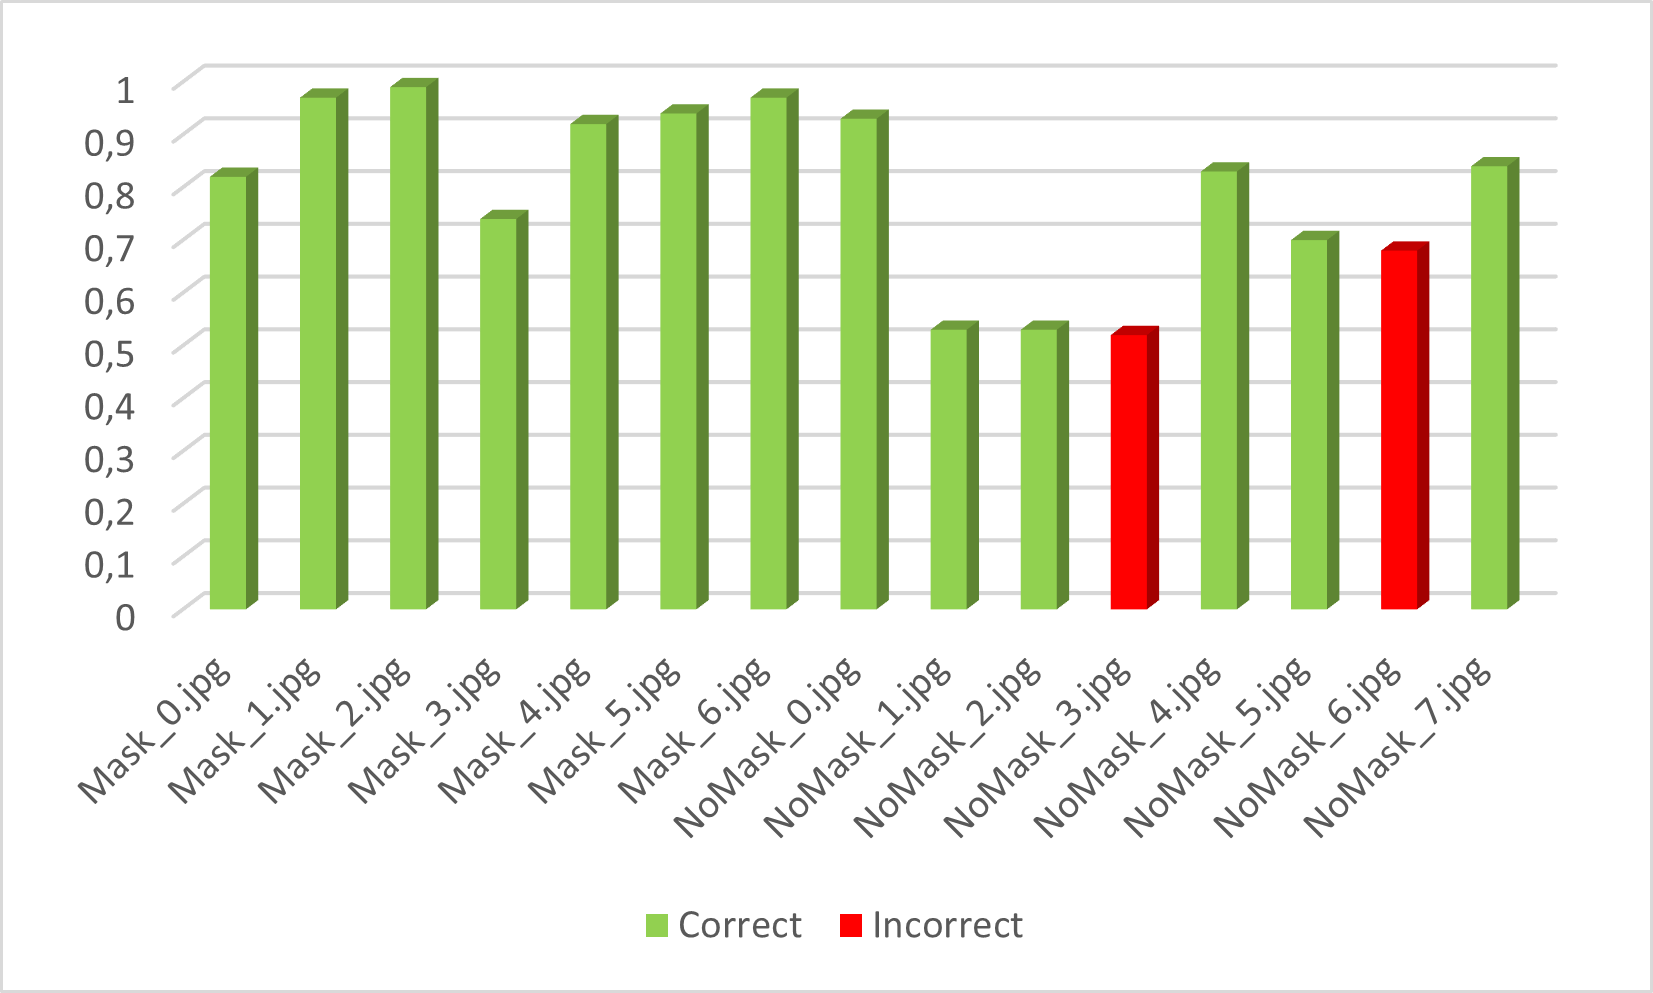
\includegraphics[width=\linewidth]{images_latex/test5_1.png}
        \caption{Model 5 - Test 1}
    \end{subfigure}
    \qquad
    \begin{subfigure}{6cm}
        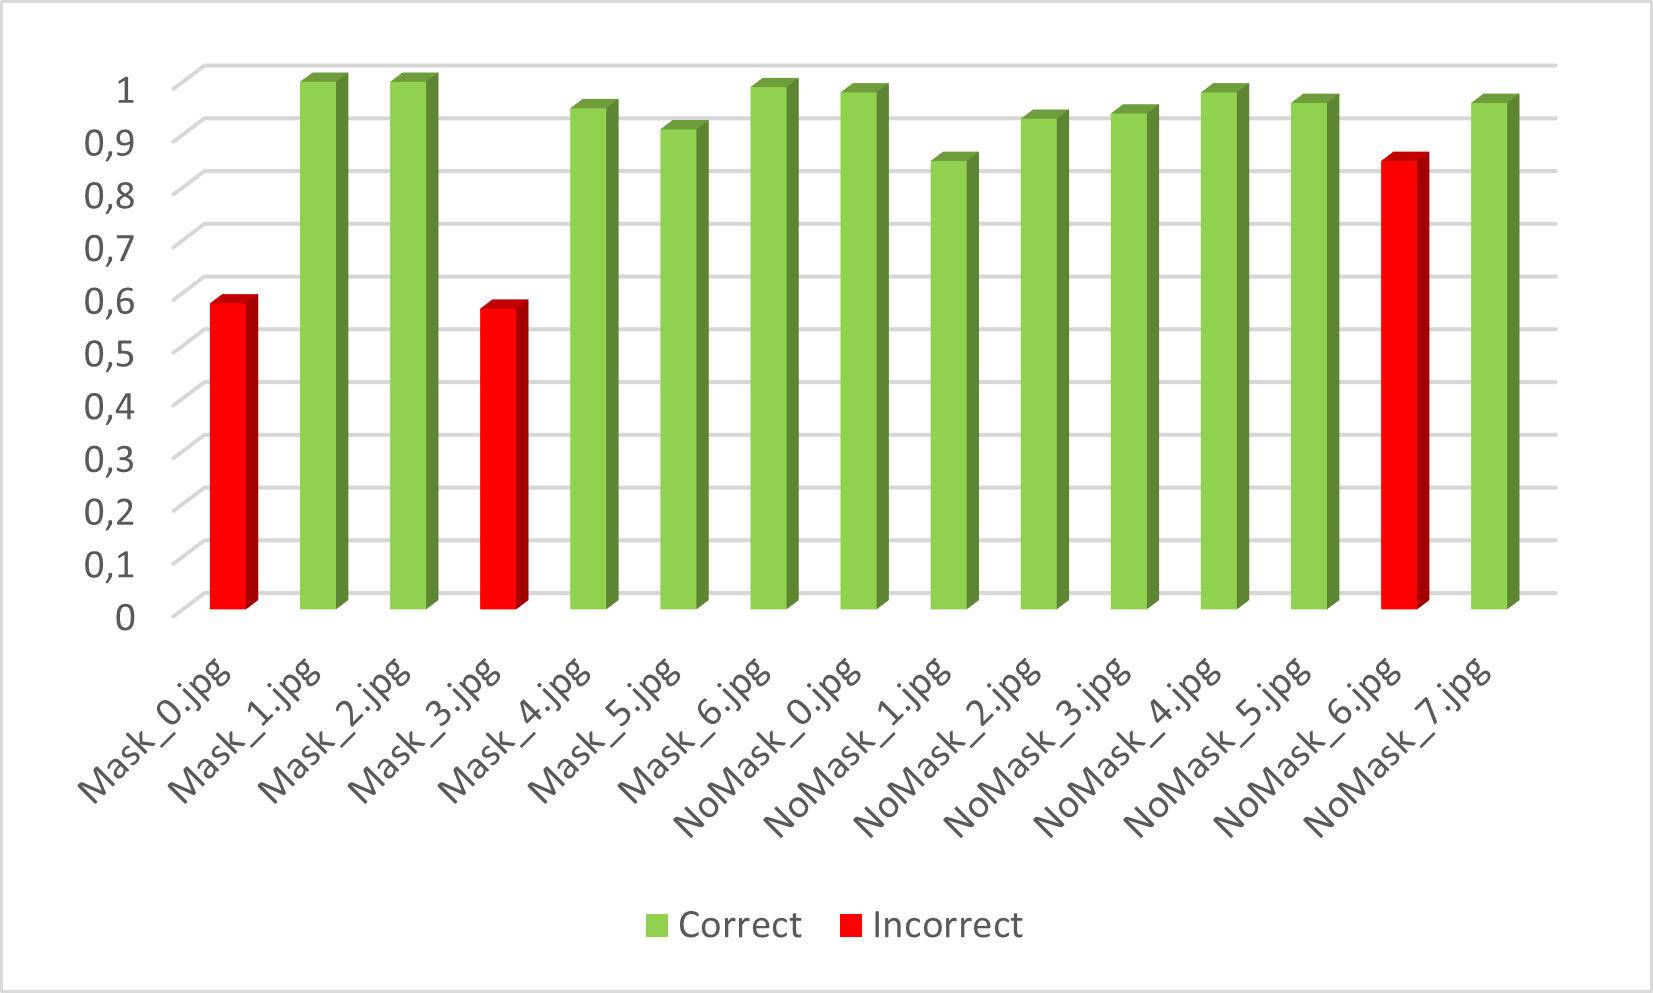
\includegraphics[width=\linewidth]{images_latex/test5_2.png}
        \caption{ Model 5 - Test 2}
    \end{subfigure}
    \qquad
    \begin{subfigure}{6cm}
        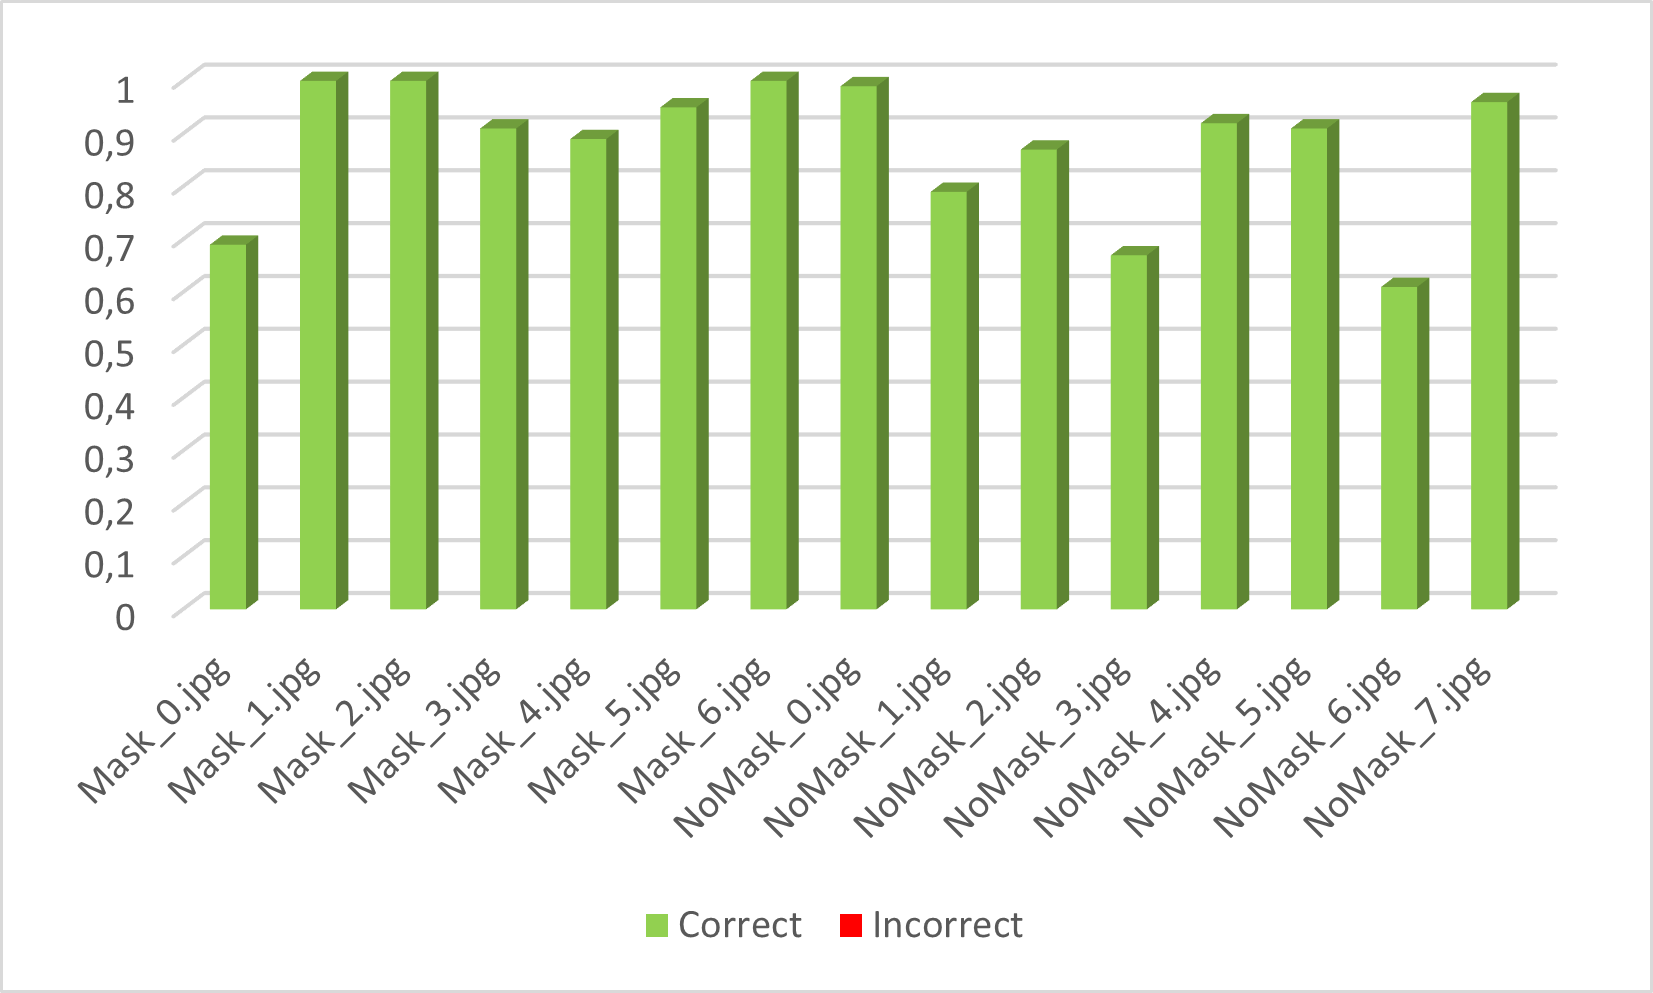
\includegraphics[width=\linewidth]{images_latex/test5_3.png}
        \caption{ Model 5 - Test 3}
        \label{fig:t5_3}
    \end{subfigure}
     \begin{subfigure}{6cm}
        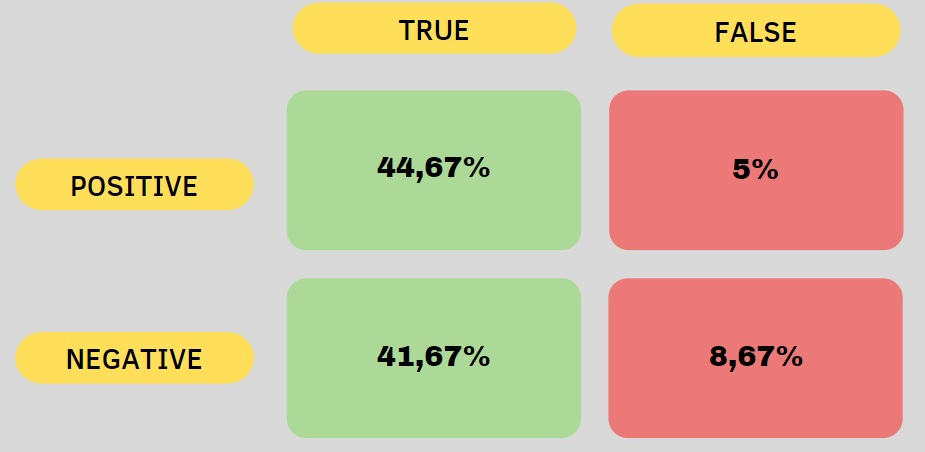
\includegraphics[width=\linewidth]{images_latex/model5.jpg}
        \caption{ Model 5 - Prediction}
    \end{subfigure}
    \caption{Scenario 5}%
\end{figure}

Given the results of the previous model, some layers have been removed and the number of channels controlled by the Conv2d layer has been decreased. 
We obtained a model that managed to get closer to a good image classification, in fact as you can see, especially in Figure \ref{fig:t5_3}, the matching Mask/Nomask is correct.
The probability in some cases reaches even 100\%, therefore this approach is the right one.
\newpage
\subsection{Model 6}

\begin{lstlisting}[
    caption={Model 6},
    label={listing:mod_6},
    mathescape=true, 
    frame=lines,
     breaklines=true,
    backgroundcolor=\color{yellow!25},
]
model  = keras.models.Sequential([
    data_augmentation,
    layers.Rescaling(1./255),
    layers.Conv2D(16, 4, padding='same', activation='relu'),
    layers.MaxPooling2D(),
    layers.Conv2D(16, 4, padding='same', activation='relu'),
    layers.MaxPooling2D(),
    layers.Conv2D(32, 4, padding='same', activation='relu'),
    layers.MaxPooling2D(),
    layers.Dropout(0.2),
    layers.Flatten(),
    layers.Dense(num_classes)
])
\end{lstlisting}

\textbf{Results}

\begin{figure}%
    \centering
    \begin{subfigure}{6cm}
        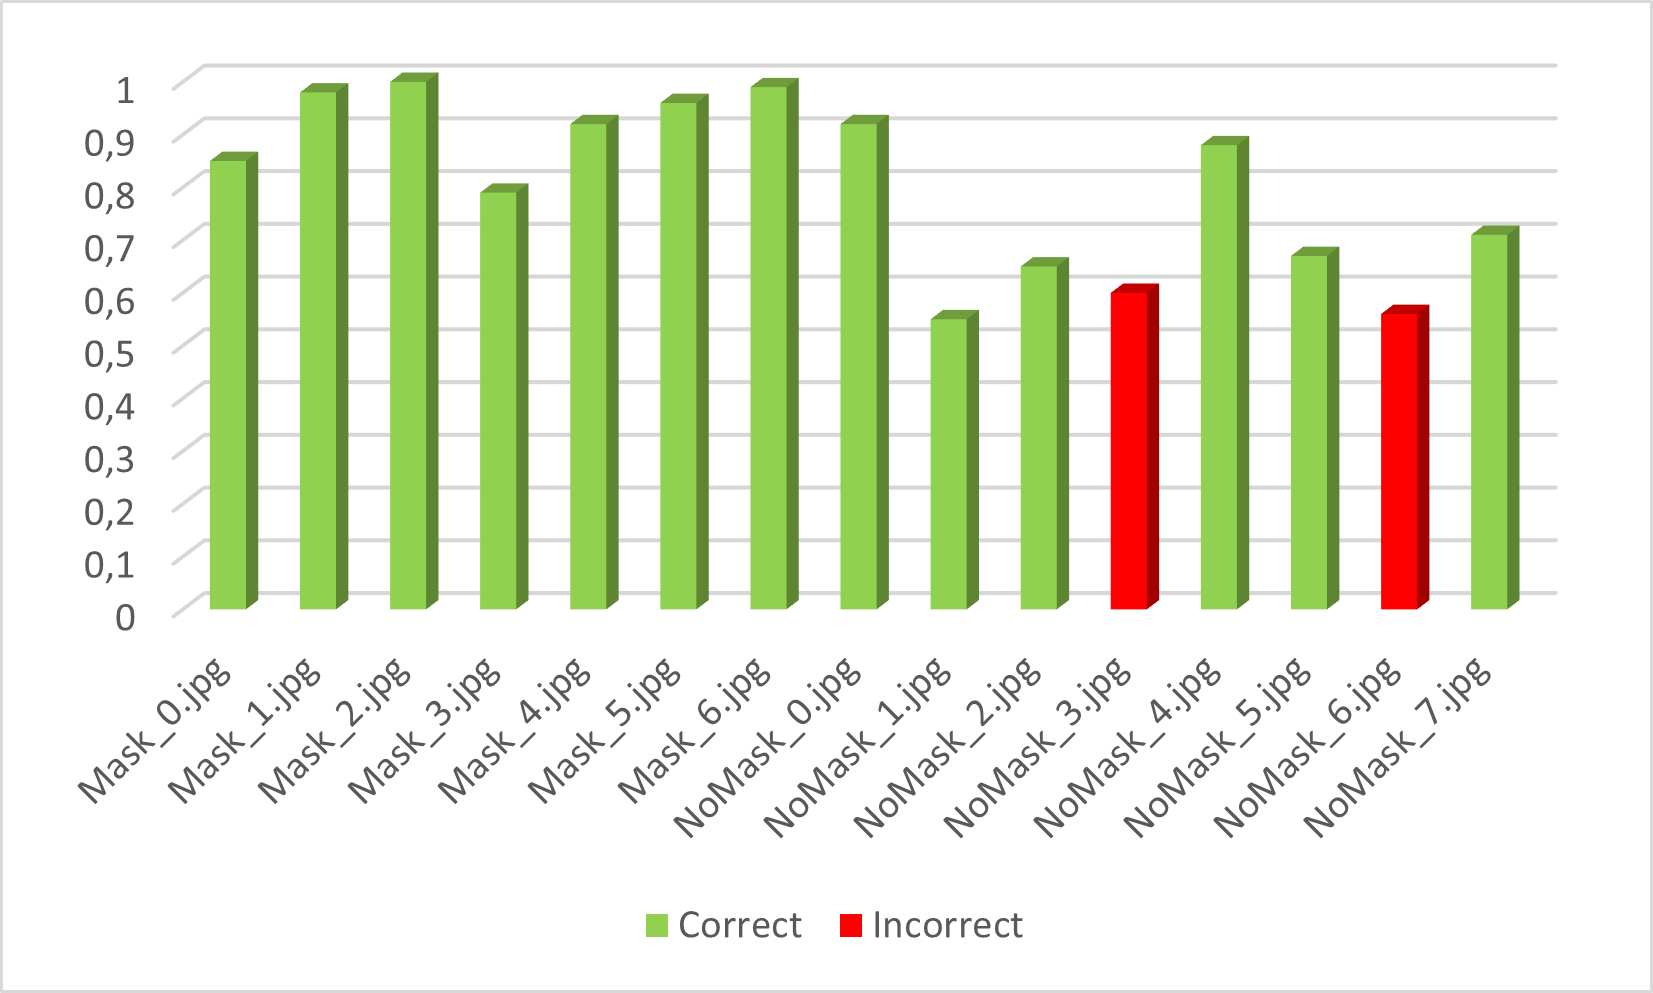
\includegraphics[width=\linewidth]{images_latex/test6_1.png}
        \caption{Model 6 - Test 1}
    \end{subfigure}
    \qquad
    \begin{subfigure}{6cm}
        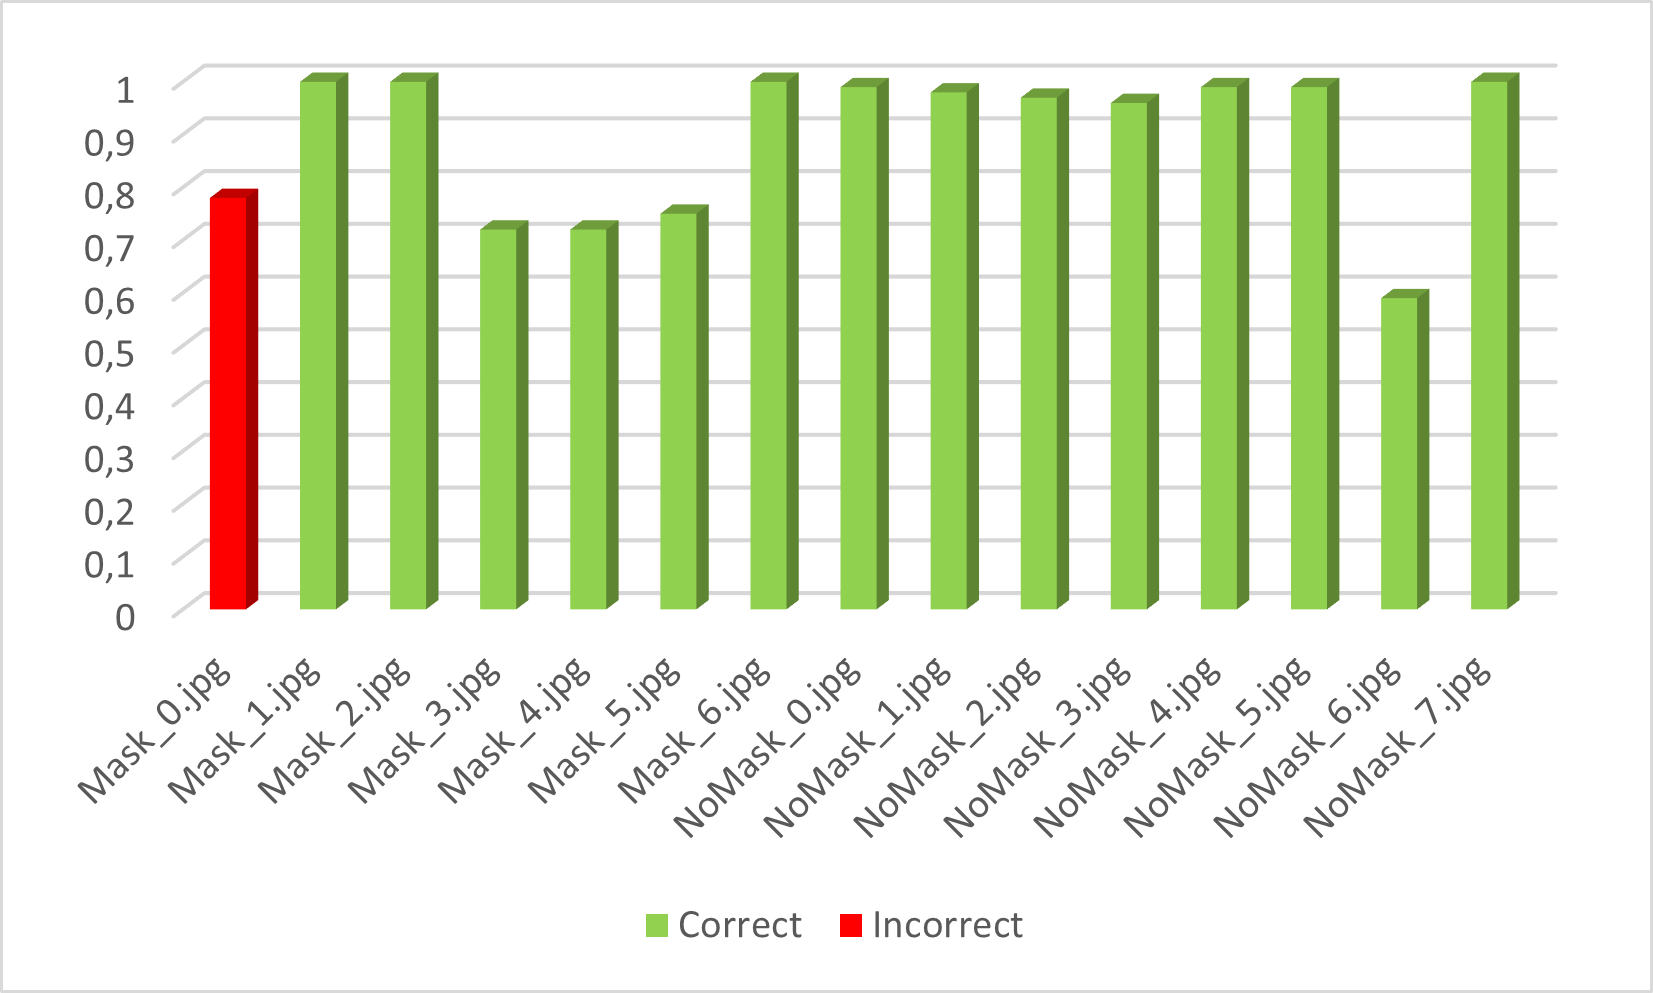
\includegraphics[width=\linewidth]{images_latex/test6_2.png}
        \caption{ Model 6 - Test 2}
    \end{subfigure}
    \qquad
    \begin{subfigure}{6cm}
        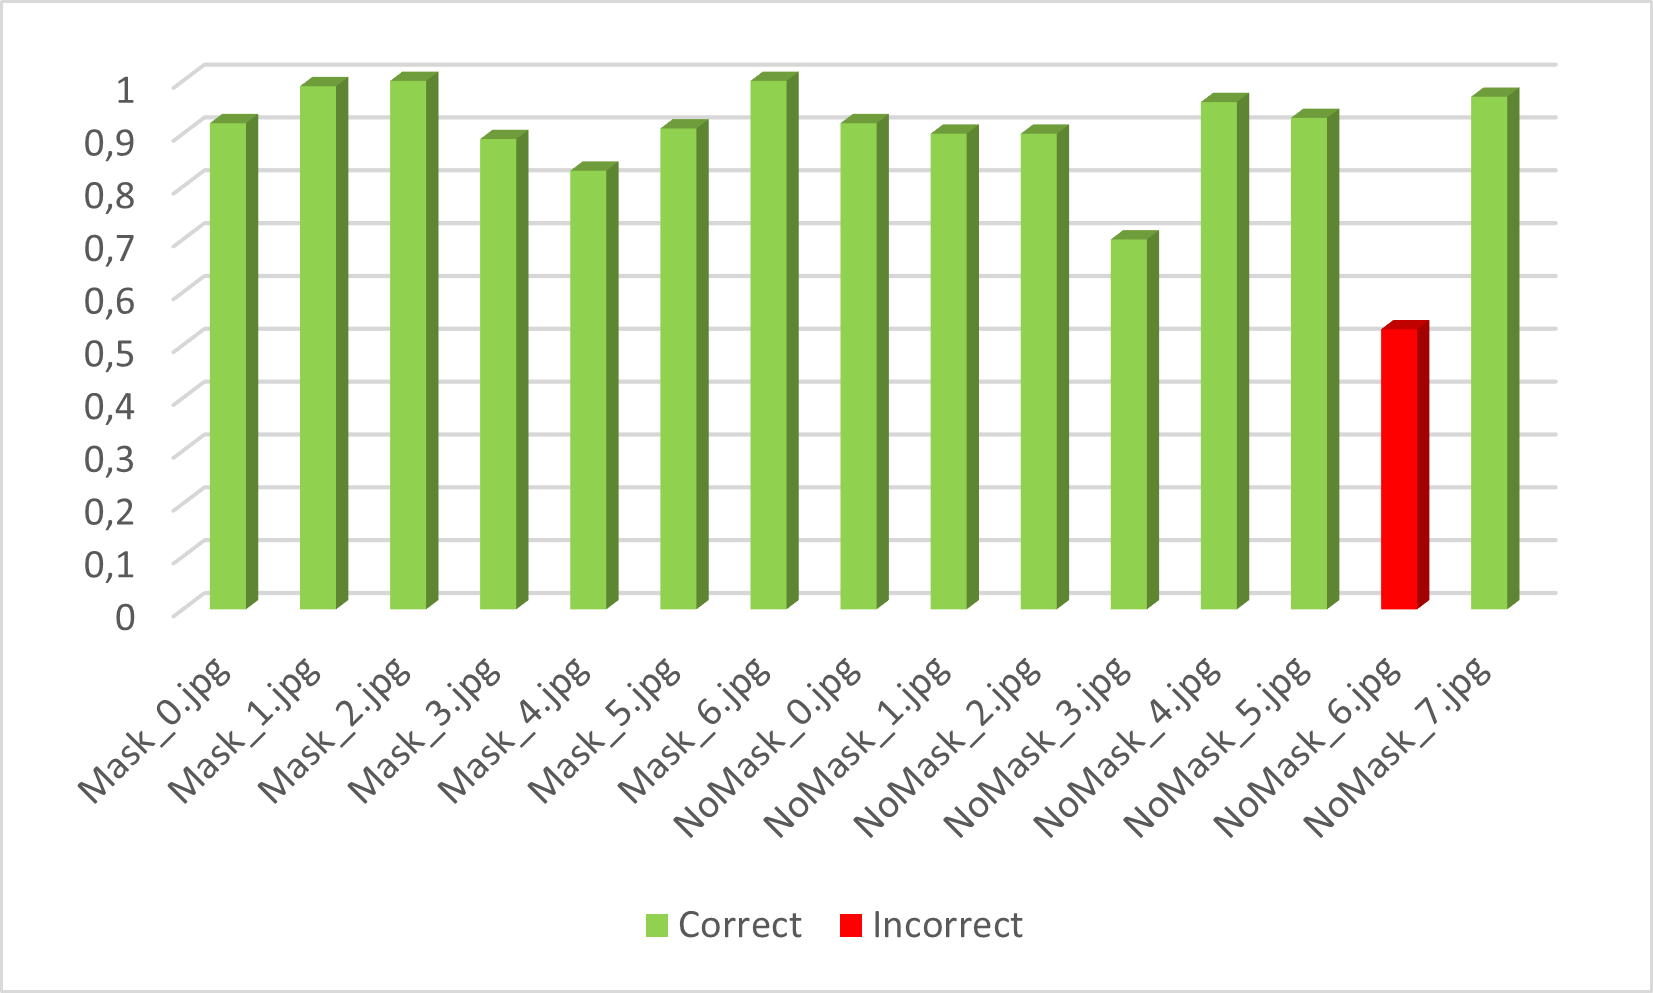
\includegraphics[width=\linewidth]{images_latex/test6_3.png}
        \caption{ Model 6 - Test 3}
    \end{subfigure}
     \begin{subfigure}{6cm}
        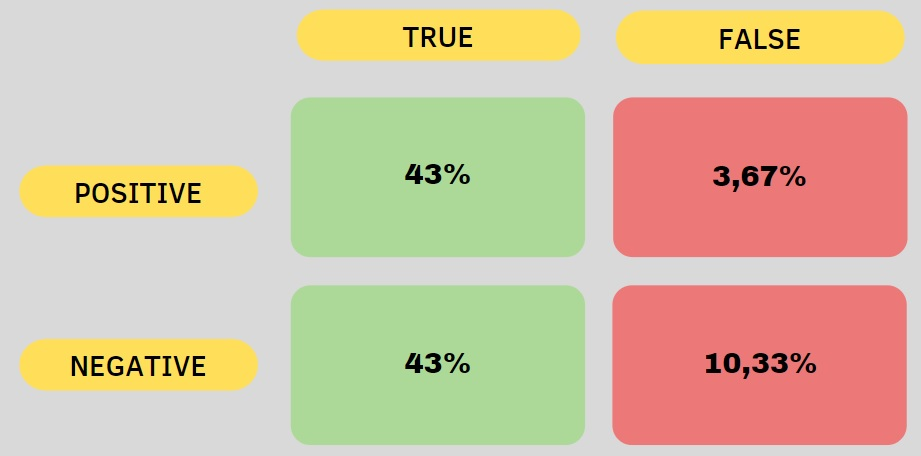
\includegraphics[width=\linewidth]{images_latex/model6.jpg}
        \caption{ Model 6 - Prediction}
    \end{subfigure}
    \caption{Scenario 6}%
\end{figure}

Adding a new Conv2D layer the results is pretty the same, but the probability is slightly lower, whereas in some cases it still reaches 100\%. 
\newpage
\subsection{Model 7}
\begin{lstlisting}[
    caption={Model 7},
    label={listing:mod_7},
    mathescape=true, 
    frame=lines,
     breaklines=true,
    backgroundcolor=\color{yellow!25},
]
model  = keras.models.Sequential([
    data_augmentation,
    layers.Rescaling(1./255),
    layers.Conv2D(16, 3, padding='same', activation='relu'),
    layers.MaxPooling2D(),
    layers.Conv2D(16, 3, padding='same', activation='relu'),
    layers.MaxPooling2D(),
    layers.Conv2D(32, 3, padding='same', activation='relu'),
    layers.MaxPooling2D(),
    layers.Conv2D(32, 3, padding='same', activation='relu'),
    layers.MaxPooling2D(),
    layers.Dropout(0.2),
    layers.Flatten(),
    layers.Dense(num_classes)
])
\end{lstlisting}

\textbf{Results}

\begin{figure}%
    \centering
    \begin{subfigure}{6cm}
        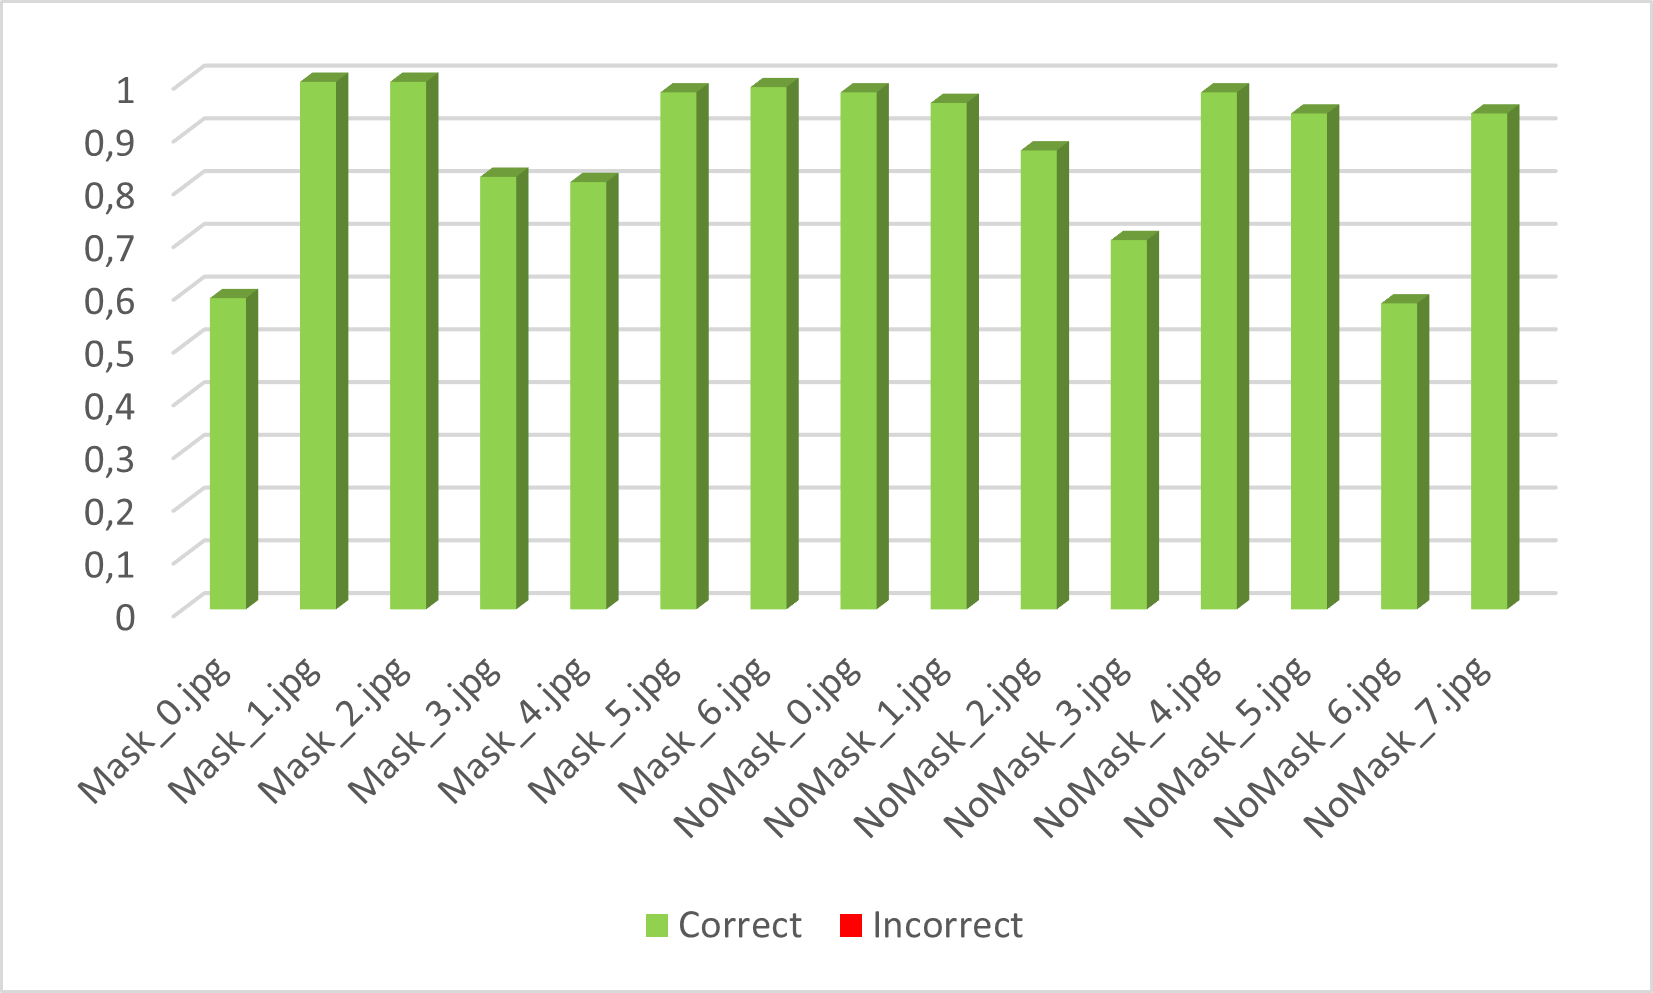
\includegraphics[width=\linewidth]{images_latex/test7_1.png}
        \caption{Model 7 - Test 1}
    \end{subfigure}
    \qquad
    \begin{subfigure}{6cm}
        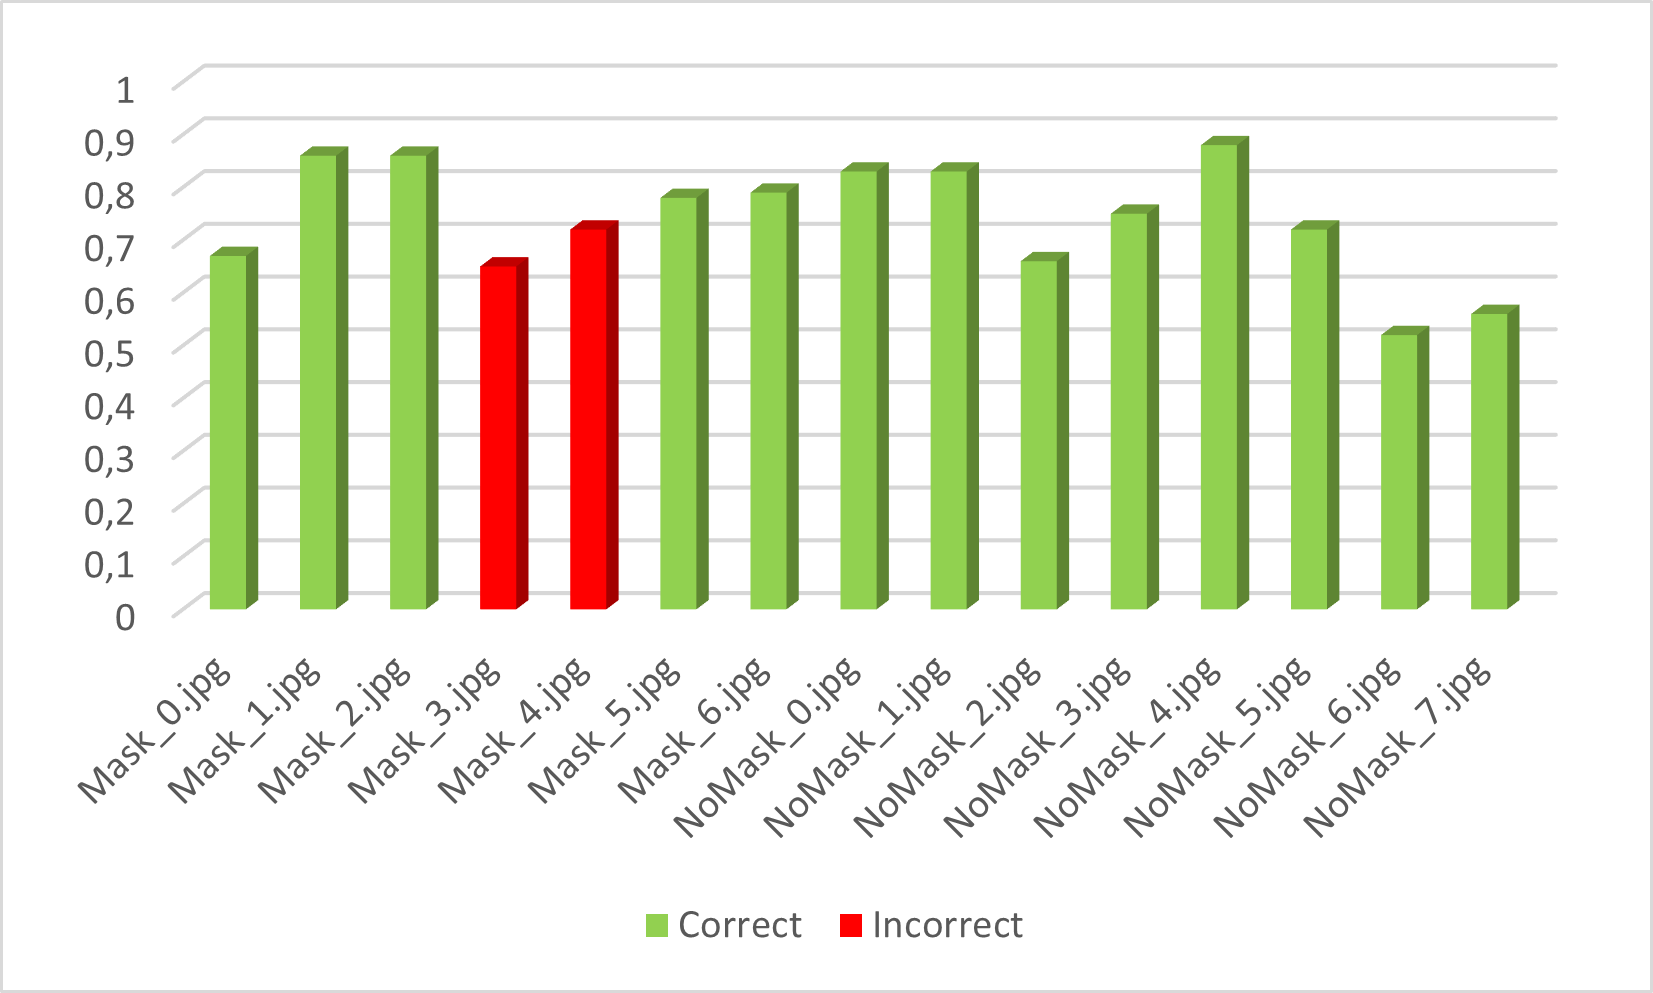
\includegraphics[width=\linewidth]{images_latex/test7_2.png}
        \caption{ Model 7 - Test 2}
    \end{subfigure}
    \qquad
    \begin{subfigure}{6cm}
        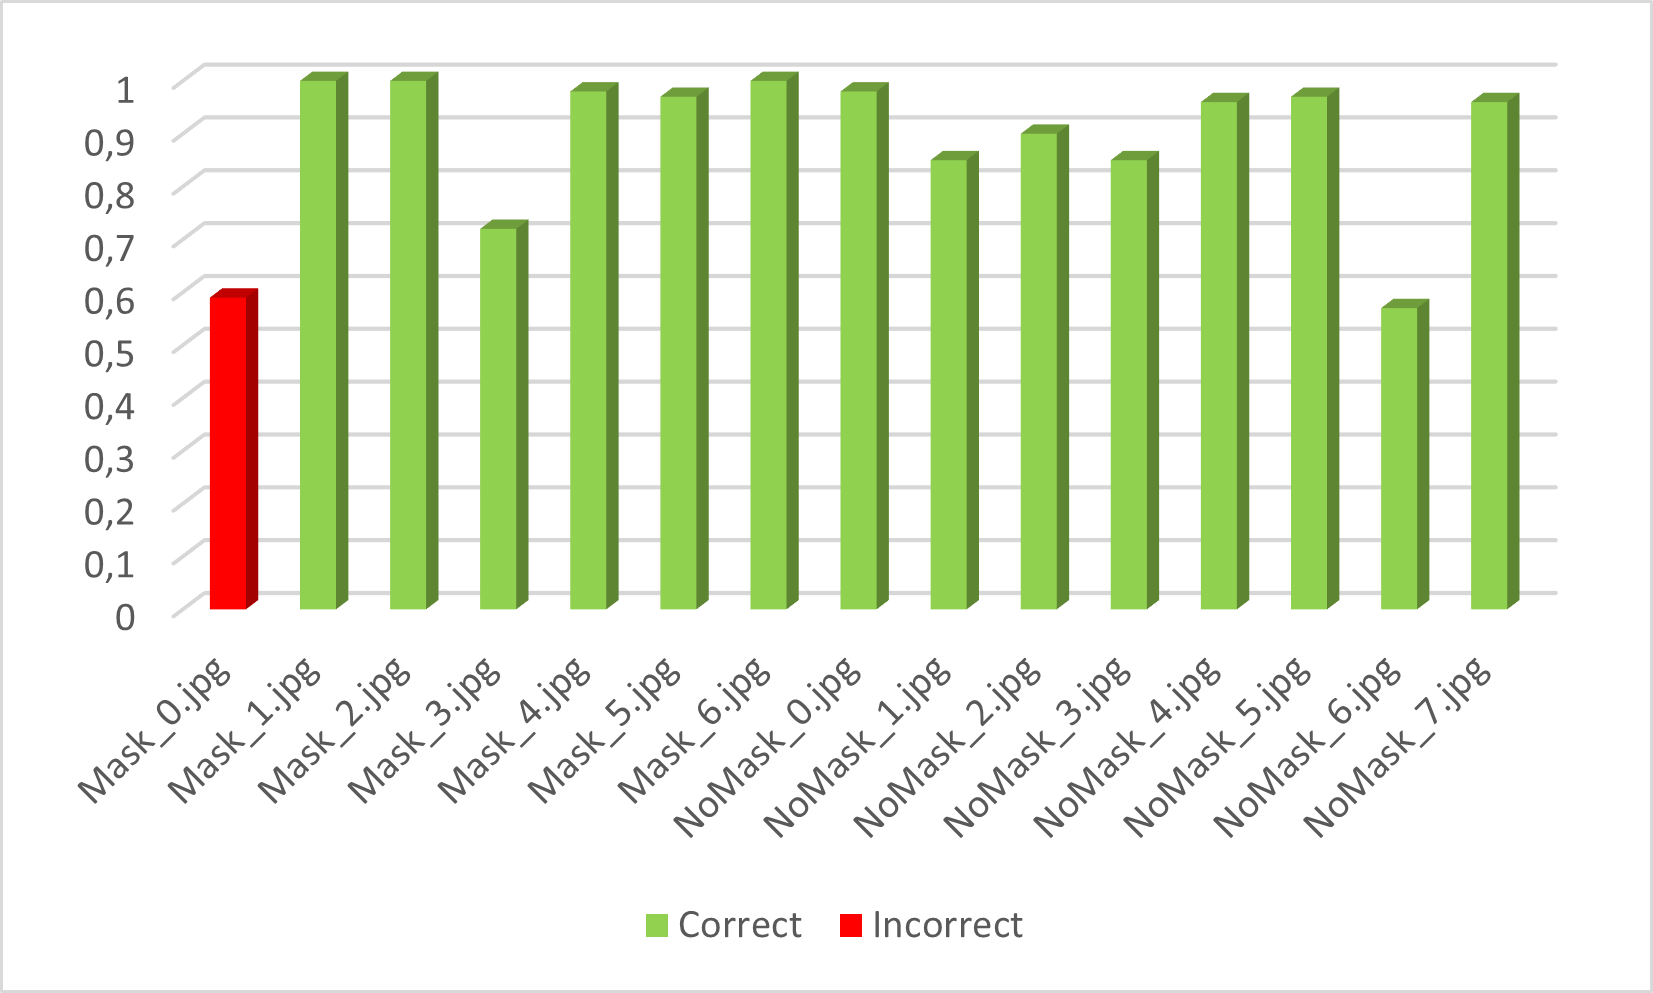
\includegraphics[width=\linewidth]{images_latex/test7_3.png}
        \caption{ Model 7 - Test 3}
    \end{subfigure}
     \begin{subfigure}{6cm}
        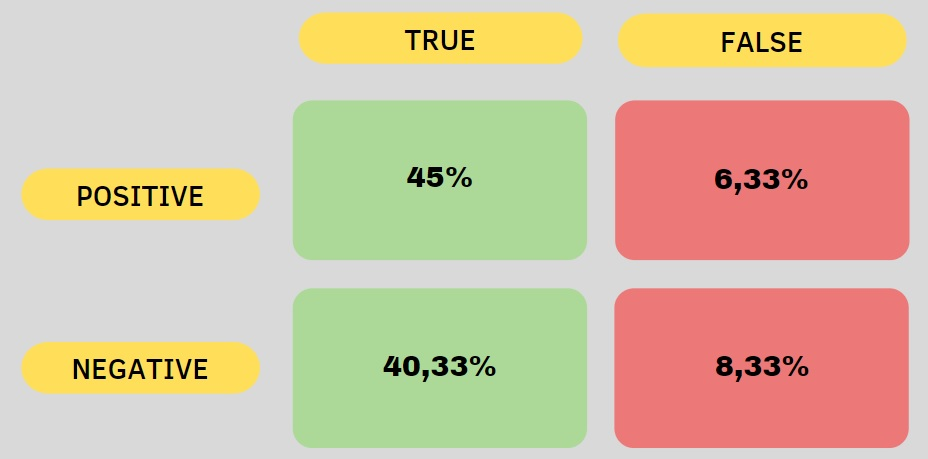
\includegraphics[width=\linewidth]{images_latex/model7.jpg}
        \caption{ Model 7 - Prediction}
    \end{subfigure}
    \caption{Scenario 7}%
\end{figure}

Proceeding in the direction of previous models, we decided to add another Conv2D layer and MaxPooling2D layer to verify if the results would improve further.
The results obtained are close to those of the sixth model, but the percentages of probability are slightly lower.

Analyzed all the seventh models, it is possible to choose those that have obtained the best results and these are the fifth, sixth and seventh models. 

In particular, the choice fell on these models because they obtained percentages close to or equal to 100\% and, in some tests, it correctly classified all the images dividing them correctly between \textit{Mask/Nomask}.

So, for future model training/testing, you could test several Conv2d, but keeping a lower value of channels controlled by the first Conv2D layer argument (in these cases 16).
\newpage
\section{Conclusion}

Finally, we have a version of our application in which we can easily manipulate and crop the images that interest us and where our intelligence is clearly able to distinguish between a person wearing a mask, and one not wearing it.

To carry out this project, we have therefore, in the first part of the project, created a functional interface to load and annotate images. We learned to use the tkinter library to place labels and menu correctly in panels and in the end we have a nice software to use. The the shapely library has been very useful and fast to easily check the area and converge different shapes such as rectangular boxes.

In the second part of the project, we realized a learning model, trained it through multiple experiments allowing us to define an image predictor which, thanks to the bounding box of the face, will classify the image in the categories \textit{Mask/NoMask}.

To compile the learning model, we use the the \textit{keras} framework and we tested a lot of different model (seven of them are cited in this report). We draw from these different tests very satisfactory results, by carrying out multiple tests for each model, we conclude that the best of our models are model 5 and 7, with 44.7\% of True Positive (resp. 45.0) and 41.7\% of True Negative (resp. 40.3).
On the contrary, some of the worst models we found are model 4 (a lot of false predictions) and model 2 (a very slow model).

The majority of the basic features have been implemented and work well, but it could be improved further by trying to find even more advanced models. Moreover, it is interesting to think that we could even consider other applications than just mask detection.

This work is finally a project that allowed us to realize how interesting it is to use the notion of neural network to identify, here in this case, a nowadays problem, the wearing of the mask and we have finally realized how complicated can be the creation of an artificial intelligence that understands what a human can detect immediately and instinctively.

\section{Bibliography}
\printbibliography

\end{document}
